\documentclass[12pt, letterpaper]{article}
%\setlength{\parindent}{0in}
\setlength{\textheight}{8.9in}
\setlength{\textwidth}{6.8in}
\setlength{\oddsidemargin}{-0.3in}
\setlength{\evensidemargin}{0.0in}
\addtolength{\topmargin}{-1in}
\setlength{\parskip}{0.1in}

\usepackage{amsmath, amsfonts}
\usepackage{graphicx}
\usepackage{caption}
\usepackage{subcaption}

\usepackage{url}
\usepackage{multirow}
\usepackage{setspace}
\onehalfspacing

\newcommand{\bmeta}{\boldsymbol{\eta}}
\newcommand{\bmtheta}{\boldsymbol{\theta}}
\newcommand{\bmbeta}{\boldsymbol{\beta}}
\newcommand{\bmphi}{\boldsymbol{\phi}}
\newcommand{\bmpi}{\boldsymbol{\pi}}
\newcommand{\bmxi}{\boldsymbol{\xi}}
\newcommand{\bmnu}{\boldsymbol{\nu}}
\newcommand{\bmmu}{\boldsymbol{\mu}}
\newcommand{\bmalpha}{\boldsymbol{\alpha}}
\newcommand{\bmzeta}{\boldsymbol{\zeta}}
\newcommand{\bmgamma}{\boldsymbol{\gamma}}
\newcommand{\bmomega}{\boldsymbol{\omega}}

\newcommand{\bmY}{\mathbf{Y}}
\newcommand{\bmZ}{\mathbf{Z}}
\newcommand{\bmX}{\mathbf{X}}
\newcommand{\bmV}{\mathbf{V}}
\newcommand{\bmW}{\mathbf{W}}
\newcommand{\bmU}{\mathbf{U}}
\newcommand{\bmR}{\mathbf{R}}
\newcommand{\bmS}{\mathbf{S}}
\newcommand{\bmb}{\mathbf{b}}

\newcommand{\bmM}{\mathbf{M}}
\newcommand{\bmSigma}{\boldsymbol{\Sigma}}
\newcommand{\bmI}{\mathbf{I}}
\newcommand{\bmTheta}{\boldsymbol{\Theta}}


\newcommand{\bea}{\begin{eqnarray}} 
\newcommand{\eea}{\end{eqnarray}} 
\newcommand{\beas}{\begin{eqnarray*}} 
\newcommand{\eeas}{\end{eqnarray*}} 
\newcommand{\benum}{\begin{enumerate}} 
\newcommand{\eenum}{\end{enumerate}} 
\newcommand{\bd}{\begin{description}}
\newcommand{\ed}{\end{description}}
\newcommand{\bi}{\begin{itemize}}
\newcommand{\ei}{\end{itemize}}

\newcommand{\mydots}{...}

\usepackage{color}
\usepackage{xcolor}

\definecolor{mygreen}{rgb}{0,0.75,0}
\definecolor{mypurple}{rgb}{0.7,0,0.8}

\newcommand{\shade}[1]{\colorbox{gray}{#1}}
%\newcommand{\highlight}[1]{\colorbox{yellow}{#1}}
\newcommand{\gbox}[1]{\colorbox{green}{#1}}
\newcommand{\tcr}[1]{\textcolor{red}{#1}}
\newcommand{\tcg}[1]{\textcolor{mygreen}{#1}}
\newcommand{\highlight}[1]{\textcolor{blue}{#1}}
\newcommand{\tcp}[1]{\textcolor{mypurple}{#1}}
\newcommand{\tcbk}[1]{\textcolor{black}{#1}}

\begin{document}

\begin{center}
\large Bayesian Joint Hierarchical Model for Prediction of Latent Health States with Application to Active Surveillance of Prostate Cancer\\
R Yates Coley, Aaron J Fisher,  Mufaddal Mamawala, H Ballentine Carter, Kenneth J Pienta, Scott L Zeger\\
August 19, 2015\\
\end{center}


\begin{center}
\textbf{Abstract}\\
In this article, we present a Bayesian joint hierarchical model for predicting a latent health state from longitudinal clinical measurements. Model development is motivated by an application to active surveillance of low risk prostate cancer. Existing joint latent class modeling approaches are unsuitable for this context as they do not accommodate measurement error-- cancer state determinations based on biopsied tissue are prone to misclassification-- nor do they allow for observations to be missing not at random. The proposed model addresses these limitations, enabling estimation of an individual's underlying prostate cancer state. We apply our model to data from a cohort of active surveillance patients at Johns Hopkins University to evaluate performance. %These individualization predictions can then be communicated to clinicians and patients to inform decision making. 
\end{center}

\section{Introduction}

Medicine is in a period of transition. An ever-increasing amount of information is available on patients ranging from genetic and epigentic profiles enabled by next-generation sequencing to moment-to-moment data collected by physical activity monitors. With this wealth of information comes the opportunity to provide more targeted health care including, for example, prediction of pre-clinical atherosclerosis \cite{McGeachie2009}, individualized cancer screening \cite{Saini2014}, sub-typing of scleroderma \cite{Saria2015},  and personalized cancer treatment\cite{Hayden2009}. In order to fully realize the promise of patient-focused medicine, principled statistical methods are needed to synthesize data from a variety of sources and provide clinicians and patients with relevant syntheses that inform decision-making. These methods must also accommodate limitations common to data generated in an observational setting including measurement error, and informative missing data patterns.


An excellent example of this challenge is low-risk prostate cancer diagnoses-- tumor lethality is an aspect of an individual's latent health state that is not directly observable but is manifest in measurements. While many measurements may be available on biomarkers, histology of biopsied tissue, genetic markers, and family history of the disease, the patient's prognosis is still uncertain. As a result, individualized predictions of the disease state can guide treatment decisions. If the tumor is potentially lethal, immediate treatment can be life-saving. Yet, some tumors are indolent and not life-threatening. In this case, treatment is not recommended due to the risk of lasting side effects including urinary incontinence and erectile dysfunction \cite{Chou2011a,Chou2011b}.


Active surveillance offers an alternative to early treatment for individuals with lower risk disease detected \cite{Carter2007, Khatami2007, Klotz2010, Soloway2008, Tosoian2011, vanAs2008, vandenBergh2009}. Though active surveillance regimes vary, the approach generally entails regular biopsies (e.g., annually) with intervention recommended upon detection of higher risk histological features, as determined by the Gleason grading system \cite{Gleason1977, Gleason1992}. Biopsies with a Gleason score of 6 indicate low risk disease while a Gleason score of 7 or above is considered \textit{reclassification} to a higher risk. Prostate-specific antigen (PSA) is also routinely measured and may be used to recommend biopsies. 

The success of active surveillance programs depend on clinicians' ability to identify tumors with metastatic potential with sufficient time for curative intervention to be effective. Biopsies used to characterize tumors, however, are only informative about the sampled tissue and, moreover, have imperfect sensitivity and specificity\cite{Epstein2012}. As a result, a biopsy does not measure the true cancer state; biopsies are instead measurements made with error. Existing clinical support tools that predict biopsy outcomes for active surveillance patients, including, most recently, Ankerst et al. (2015)\nocite{Ankerst2015}, contribute valuable information to guide decisions about biopsy timing and frequency but are insufficient to address patients' primary concerns. Instead, patients and clinicians would prefer prediction of the pathological make-up of the entire prostate, including any presence of higher risk features, in order to guide decision-making.

With this application in mind, we have developed a Bayesian hierarchical model that enables prediction of an individual's underlying disease status via joint modeling of repeated PSA measurements and biopsies. Specifically, we predict a binary cancer state- \textit{indolent} or \textit{aggressive}- with the latter defined as an actual Gleason score of 7 or higher. Predictions are informed by a subset of patients for whom the true state is observed-- patients who, either before or after reclassification, underwent elective prostatectomy. In this sense, cancer state operates as a partially-latent class in the proposed model \cite{Wu2015}. 

An individual's cancer state influences both the level and trajectory of PSA measurements as well as the outcomes from repeated biopsies. These relationships are illustrated by the directed acyclic graph (DAG) in Figure 1(a). In the model we are proposing, PSA measurements follow a mixed effects model with mean effects varying across latent classes \cite{Laird1982}. Then, biopsy outcomes, a binary indicator of reclassification at each year of follow-up, are modeled with a pooled logistic regression model under the assumption that biopsy results are independent conditional on cancer state and covariates (age, time since diagnosis, etc.)\cite{Cupples1988,D'Agostino1990}. As codified in the Figure 1(a) DAG, PSA and biopsy results are also assumed to be conditionally independent given latent class. 

\begin{figure}
\begin{center}
%\begin{subfigure}[b]{0.3\textwidth}
%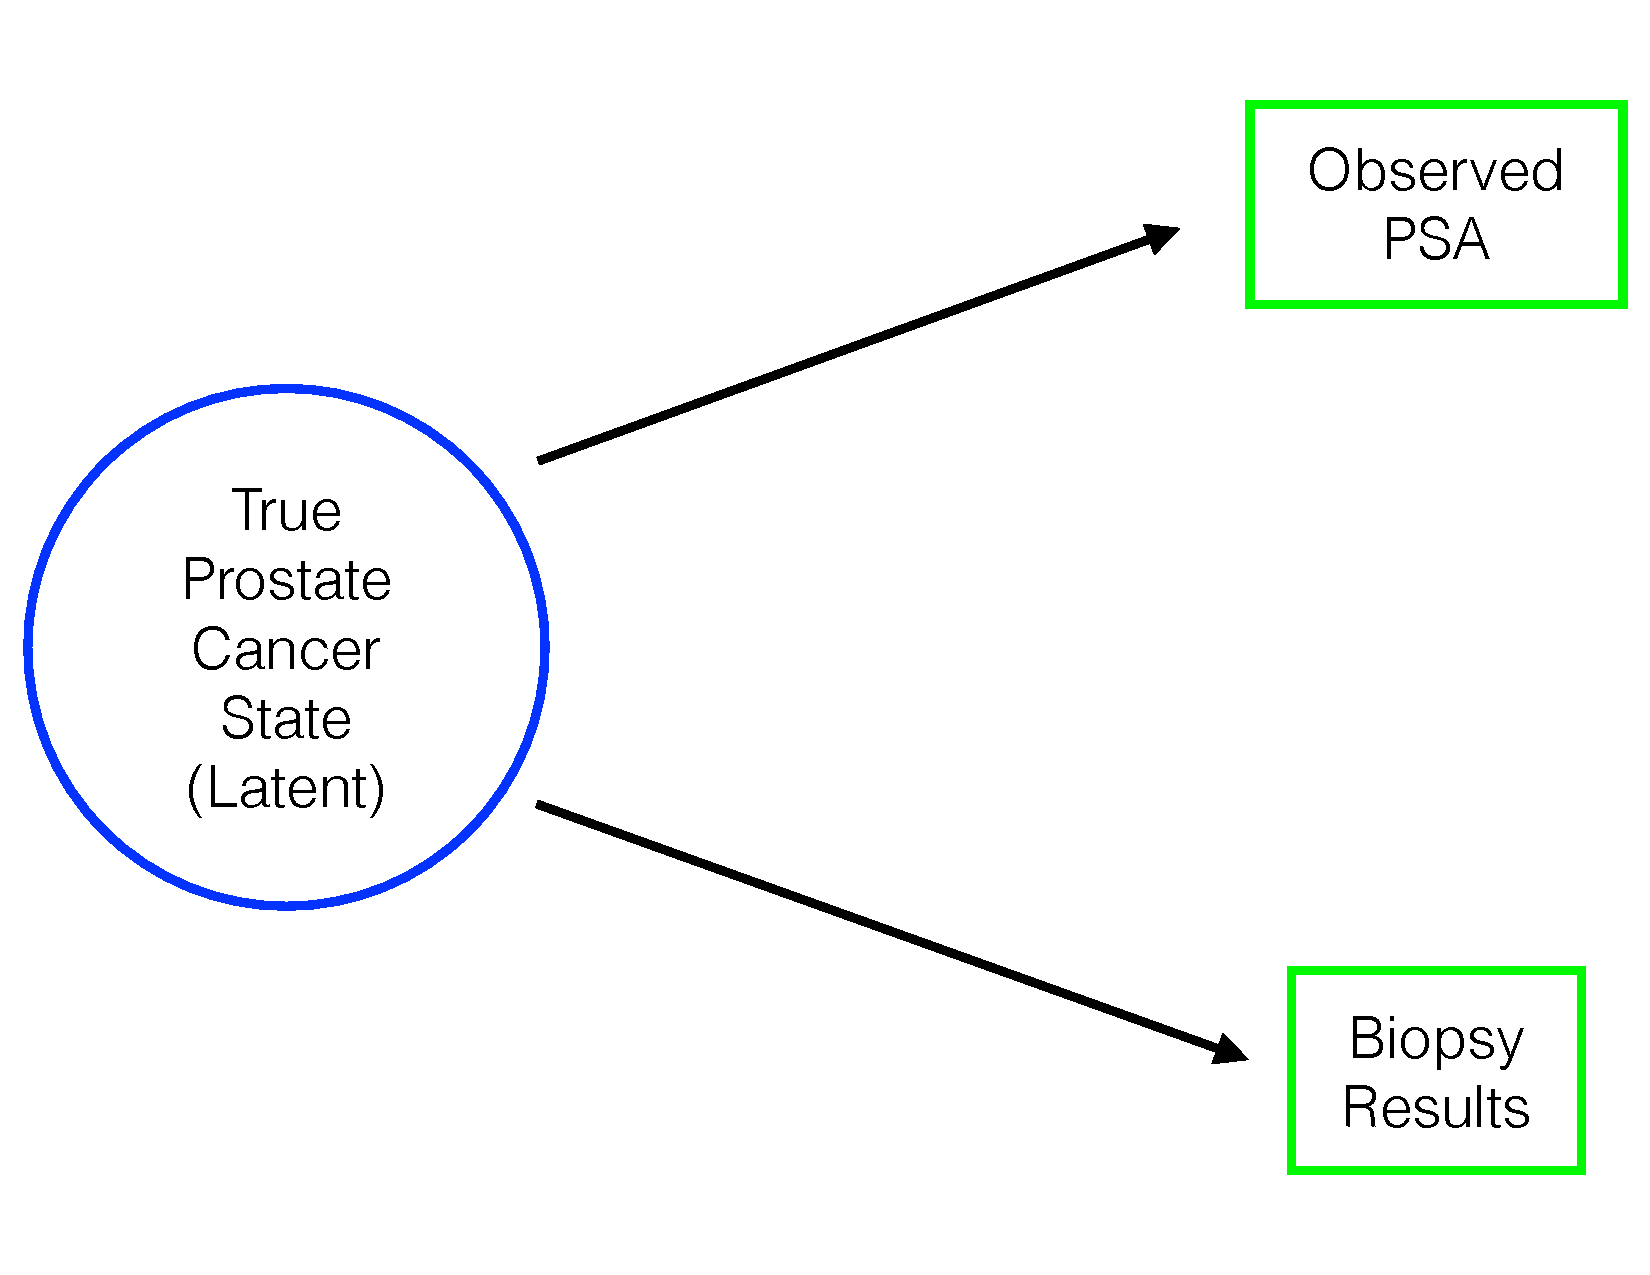
\includegraphics[width=\textwidth]{dag1}
%\caption{}%Time Point Joint Model}
%\label{fig:dag1}
%\end{subfigure}
\begin{subfigure}[b]{0.45\textwidth}
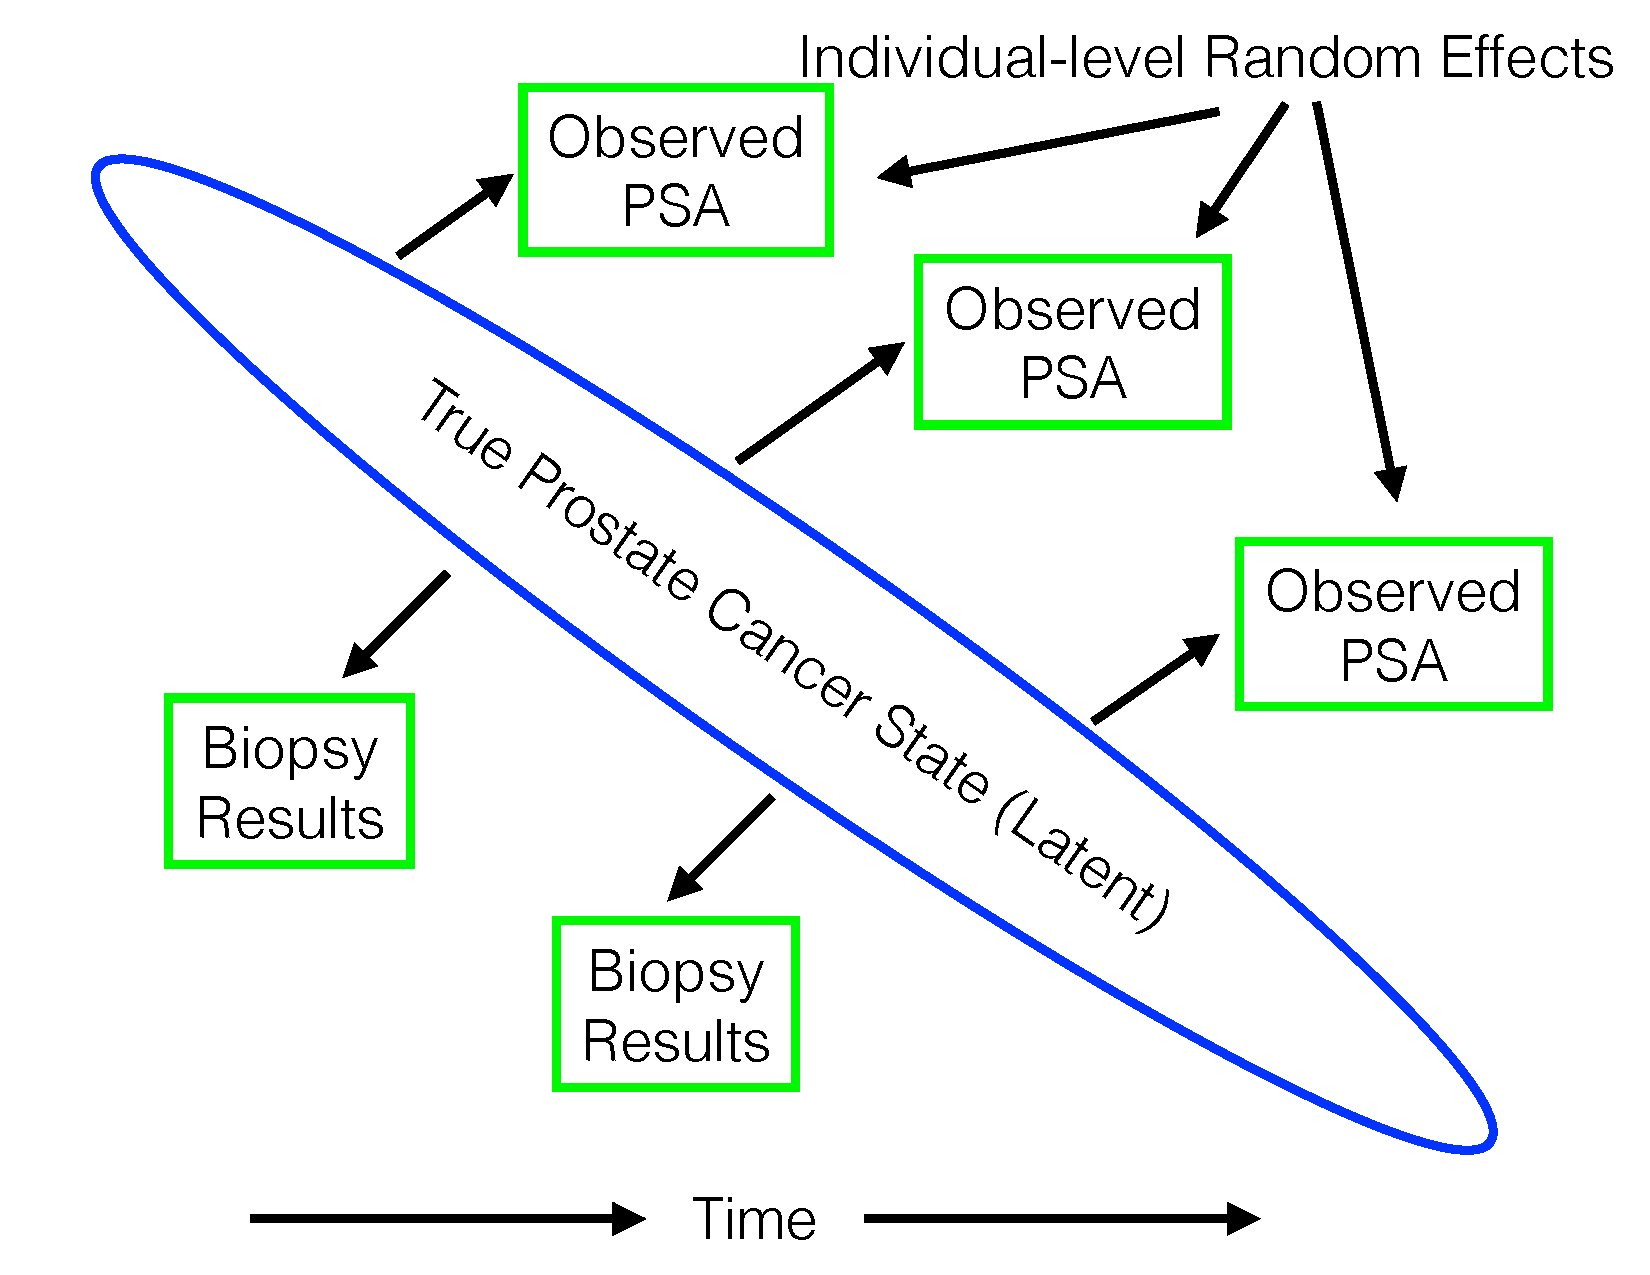
\includegraphics[width=\textwidth]{dag2}
\caption{}%Time-Varying Joint Model}
\label{fig:dag2}
\end{subfigure}
\begin{subfigure}[b]{0.45\textwidth}
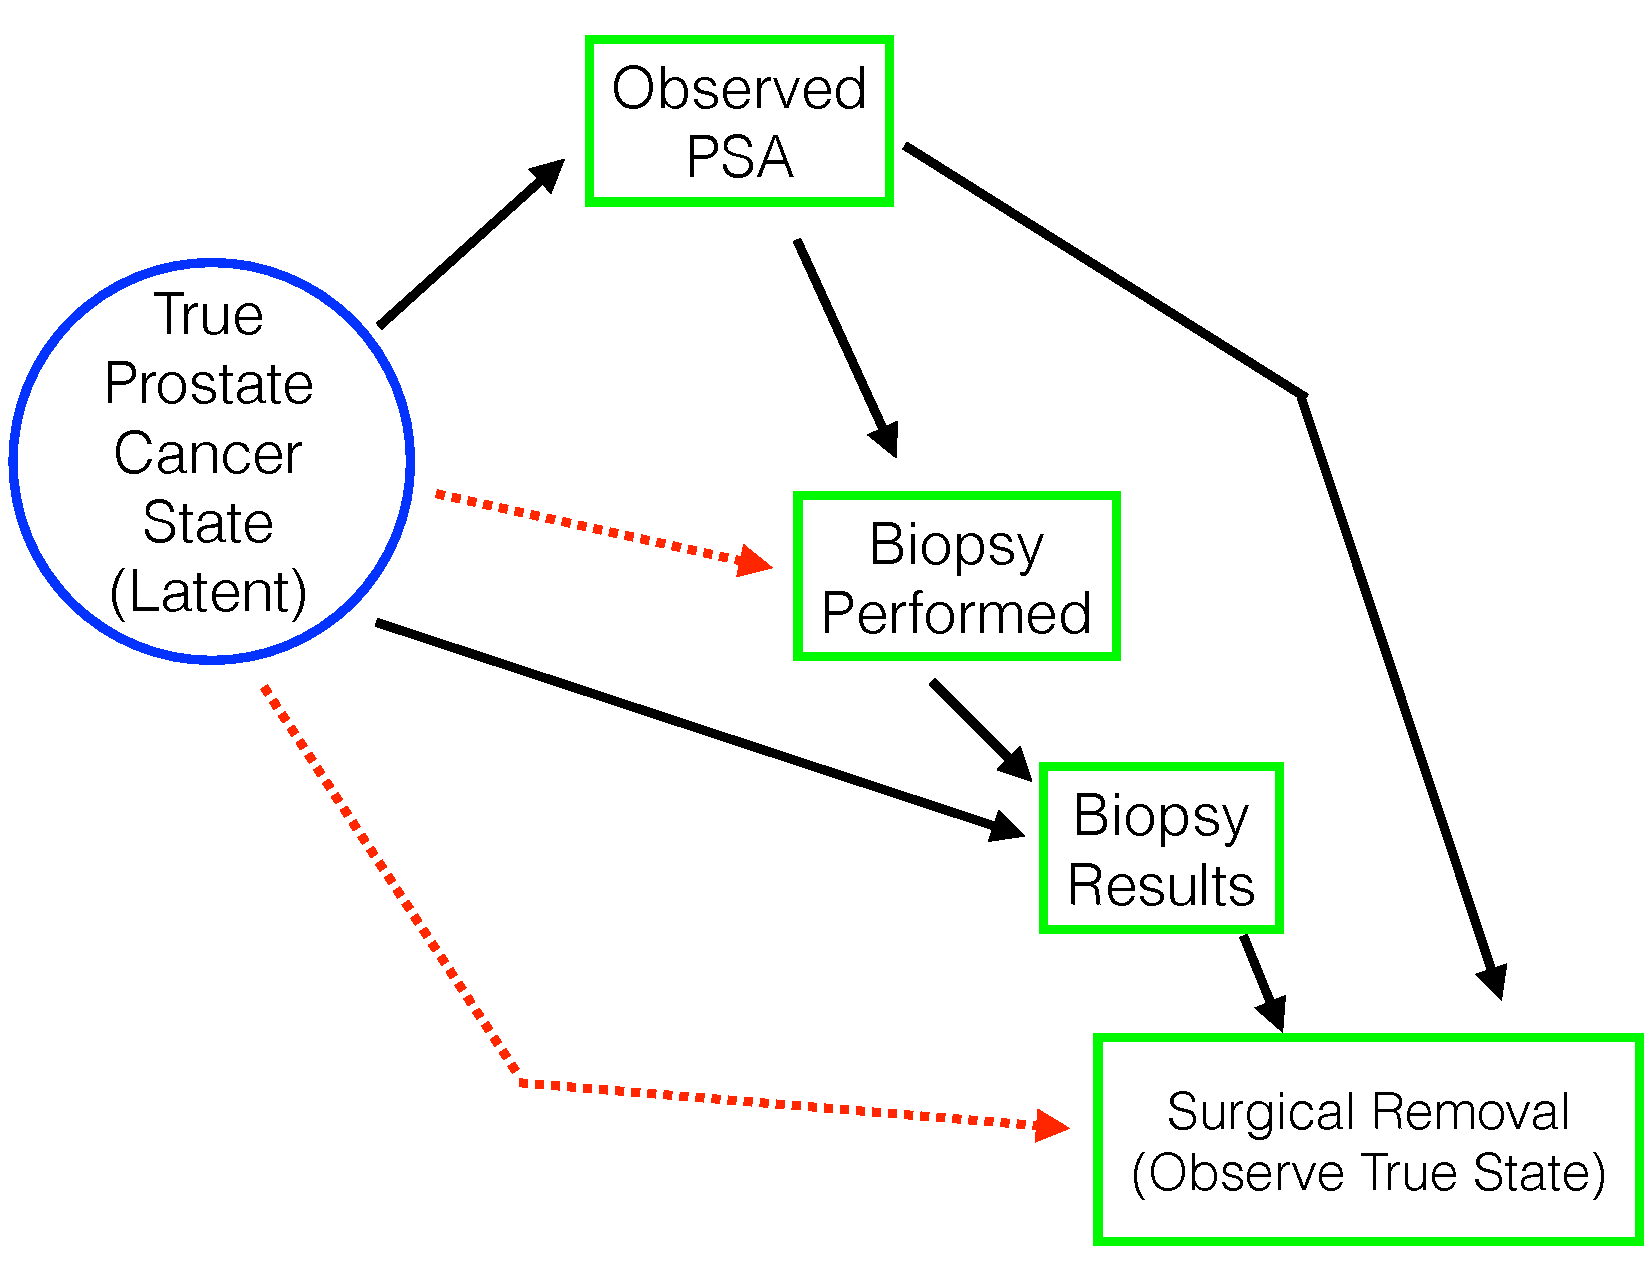
\includegraphics[width=\textwidth]{dag3}
\caption{}%Informative Observation Process}
\label{fig:dag3}
\end{subfigure}
\caption{DAGs describing the relationships between latent class (circled) and observed measurements (squared) (a) over time and (b) in the presence of an informative observation process (at a single time point).}
\end{center}
\end{figure}

This first model is related to previous work by Lin et al. (2002)\nocite{Lin2002}, who proposed a joint latent class model (JLCM) to analyze longitudinal PSA and time-to-diagnosis of prostate cancer, extending developments in joint models by Schluchter (1992)\nocite{Schluchter1992}, DeGruttola and Tu (1994)\nocite{DeGruttola1994}, and Henderson, Diggle, and Dobson (2000)\nocite{Henderson2000}. The JLCM has since been applied in many settings, including an extension of the method by Proust-Lima and Taylor (2009)\nocite{Proust2009} to develop a dynamic prognostic tool for prostate cancer recurrence after radiation therapy. Use of JLCM is motivated by interest in modeling differential risk and disease progression across a population and classifying individuals with similar outcomes, but, unlike our approach, does not involve a priori specification of classes of interest. 

Motivated by the active surveillance problem, the method proposed here addressed the limitations of JLCM and advances the development of latent variable models for multivariate outcomes in two ways. First, the proposed joint model accommodates inherent measurement error when monitoring disease progression. Second, our model is more appropriate for a clinical context where time-to-disease progression depends on non-random observation times. Among patients with low risk disease, presentation of symptoms is rare and the timing of biopsies is instead influenced by AS protocol and observed PSA results. To this latter point, the conditional independence assumption in JLCM is suspect as observation of a high PSA increases the chance of a biopsy. The proposed model addresses this limitation by modeling reclassification with a pooled logistic regression model \cite{Cupples1988, D'Agostino1990} and conditioning on the presence of a biopsy. 

Our approach also allows the occurrence of a biopsy and surgical removal of the prostate to depend on the latent cancer state. Absent a biopsy or surgery, we do not observe the biopsy results or true cancer state, respectively. If we treat this information as missing, our extension is to allow missing not at random (MNAR) data with missing at random (MAR) as a special case \cite{Little2014}. Consider the dotted lines in the DAG in Figure 1(b)-- if true cancer state is associated with the choice to perform a biopsy or undergo surgery after conditioning on observed PSA and biopsy results, then informative missingness is present and predictions will be biased \cite{Wu1988}. In response, we propose including cancer state as a predictor in regression models for the probability having a biopsy and having surgery at each annual interval. In this way, the dependence between observing the outcome and its value is accommodated.
This approach is similar to the latent class dropout model, proposed by Roy (2003, 2007)\nocite{Roy2003,Roy2007}, a type of shared parameter model \cite{Follmann1995} with discrete random effect. Unlike Roy's model for intermittent missingness which models latent class conditional on the observation process, we follow the model formulation outlined in Albert and Follmann (2009)\nocite{Albert2009}, specifying distributions for the outcome and the observation process conditional on cancer state.

%Additionally, in order to support decision-making in a clinical setting, we have developed an importance sampling algorithm to enable real-time updating of model predictions \cite{Geweke1989}. 


This paper is organized as follows. In Section 2, we describe data from an active surveillance cohort at Johns Hopkins. A joint hierarchical model for latent class prediction is outlined in Section 3, including a description of Bayesian estimation procedures. Section 4 presents an application of the model to the active surveillance cohort. We close with a discussion.
%Then, importance sampling methods to obtain quick predictions update are detailed and demonstrated in Section 5.

\section{Active Surveillance Program for Prostate Cancer at Johns Hopkins}
From January 1995 to June 2014, the Johns Hopkins Active Surveillance cohort has enrolled 1,298 prostate cancer patients \cite{Tosoian2015}. In this study, patients with very-low-risk or low-risk prostate cancer diagnoses (according to criteria outlined in Epstein et al. (1994)\nocite{Epstein1994}, including biopsy Gleason score of 6) who elect to delay curative intervention in favor of active surveillance are followed prospectively. Characteristics of diagnostic biopsy and results of all prior PSA tests are collected at enrollment. As part of the surveillance regimen, PSA tests are typically performed every six months, and biopsies are performed annually, though these intervals vary; the results of all tests are recorded. Curative intervention is recommended upon biopsy grade reclassification, that is, when the Gleason score assigned to a biopsy exceeds 6. (Volume reclassification can also occur, but we grade reclassification is the focus of this paper.) Some patients also choose to undergo curative intervention prior to reclassification. For patients who elect surgical removal of the prostate (whether prior to or after reclassification), Gleason score determination based on full pathologic analysis of the prostate specimen is also recorded.

\section{Joint Hierarchical Latent Class Model}

We have developed a Bayesian, joint hierarchical model of the underlying cancer state, measurement process, and outcomes of patients enrolled in active surveillance. Predictions are made by incorporating information from repeated PSA and biopsy measurements for all individuals, as well as true cancer state information observed in a potentially non-random subset of the cohort. Predictions are also informed by the presence of some observations, which we refer to as an \textit{informative observation process} (IOP). In this section, we introduce notation and models for the latent state, outcome measurements, and IOP and then define the likelihood in terms of these components. We then complete Bayesian specification of the model by identifying appropriate priors and defining the joint posterior distribution. Model structure is summarized in Figure \ref{fig:model-summary}.

%\subsection{}

Define individual $i$'s true cancer state, $\eta_i$, as either indolent, $\eta_i=0$, or aggressive, $\eta_i=1$, $i=1,\dots,n.$ We use the Gleason score that would be assigned if his entire prostate were to be removed and pathologic analysis performed to define $\eta_i=0$ if Gleason $\leq$6 and $\eta_i=1$ if Gleason $\geq$ 7. True cancer state is then modeled as a Bernoulli random variable, $\eta_i \sim Bern(\rho)$, where we assume a shared underlying probability of aggressive cancer, $\rho$, for simplicity in initial presentation. Since we observe this true cancer state on a subset of patients in active surveillance who choose surgical removal of the prostate, $\eta_i$ is a partially observed latent variable. 

Next, we consider PSA, which is influenced by the true cancer state as well as age, prostate volume, and other sources of inflammation. Imprecise measurements of PSA are observed at randomly selected points in time. We use a mixed effects model to model the anticipated trajectory of an individual's PSA over time \cite{Laird1982}. Mean effects for predictors are allowed to vary across groups defined by the partially latent true cancer state as follows: 
\beas
\big[\, Y_{im} | \eta_i=k, \bmX_{im}, \bmZ_{im}\,\big] = \bmX_{im}\bmbeta + \bmZ_{im}\bmb_i + \epsilon_{im}
\eeas
where $Y_{im}$ is the observed (log-transformed) PSA, $\bmX_{im}$ and $\bmZ_{im}$ are vectors of covariates for individual $i$'s $m$th PSA measurement, $\bmbeta$ is a parameter vector for fixed effects, and $\bmb_i$ is the patient-specific vector of random effects. Following the specification of a Bayesian mixed effects model presented by Gelman and Hill (2006)\nocite{Gelman2006}, unscaled random effects are centered at the mean effects for each latent class $k$, $\bmmu_k$:
\beas
\big[\check{\bmb_i} | \eta_i=k\big] \sim MVN ( \bmmu_k, \Sigma_k), \quad k=0,1 
\eeas
where $\Sigma_k$ is a covariance matrix that allows for correlation between random effects. Random effects are then scaled with parameter vector $\bmxi$: $\bmb_i = diag(\check{\bmb_i}\bmxi^T)$. Lastly,
residuals $\epsilon_{im}$ are assumed to follow a normal distribution with mean 0 and variance $\sigma^2$. 

%The results of biopsies performed while in AS 
We then consider information about the true cancer state contained in the presence and results of prostate biopsies. Biopsy data are categorized into discrete time intervals with $(B_{ij}, R_{ij})$ denoting binary variables for individual $i$ in time interval $j$ indicating whether a biopsy was performed and, when it was, if reclassification was observed, respectively. $(B_{ij}, R_{ij})$ is defined for $j=1,\dots, J_i$ where $J_i$ is the time of reclassification or censoring for patient $i$. For each time interval, we use logistic regression to model the presence of a biopsy and, when a biopsy is performed, its result conditional on true cancer state:
\bea
\label{eq:p_bx}
P(B_{ij}=1 | \eta_i=k, \bmU_{ij}, \bmnu) = \text{logit}^{-1}\big( \bmU_{ij}(k) \bmnu \big)\\
\label{eq:p_rc}
P(R_{ij}=1 | B_{ij}=1, \eta_i=k, \bmV_{ij}, \bmgamma) = \text{logit}^{-1}\big( \bmV_{ij}(k)\bmgamma \big)
\eea
where $\bmU_{ij}(k)$ and $\bmV_{ij}(k)$ are matrices of time-varying predictors including $\eta_i$ and $\bmnu$ and $\bmgamma$ are parameter vectors. This model specification reflects two relevant aspects of data generated in AS: first, whether or not a biopsy is performed may be informative of true cancer state, and second, reclassification on biopsies is prone to measurement error.

Lastly, to allow for the possibility that surgical removal of the prostate, and subsequent observation of the true cancer state, is informative, surgery data is included in the joint model. We define $S_{ij}$, a binary indicator of surgery for individual $i$ during time interval $j$ for $j=1,\dots,J_{S_i}$, where $J_{S_i}$ is the time of surgery or other censoring for patient $i$. We model the time-to-surgery using a pooled logistic regression model with the probability of surgery in each time interval defined as:
\beas
P(S_{ij}=1 | \eta_i=k, \bmW_{ij}, \bmomega) = \text{logit}^{-1}\big( \bmW_{ij}(k)\bmomega \big)
\eeas
where $\bmW_{ij}(k)$ is a matrix of time-varying predictors including cancer state $\eta_i=k$ and $\bmomega$ is a parameter vector. 


Having specified models for each information source, we define the joint probability of the parameters given data and unobserved latent variables:

\bea
&&L\Big(\rho, \bmbeta, (\bmmu_k, \Sigma_k), \bmnu, \bmgamma, \bmomega \, | \,\big( \eta_i, (\bmY_i, \bmb_i, \underline{\bmX_i}, \underline{\bmZ_i}), (\mathbf{B}_{i}, \underline{\bmU_{i}}), (\mathbf{R}_{i}, \underline{\bmV_{i}}), (\mathbf{S}_{i}, \underline{\bmW_{i}}) \big), i=1,\mydots,n \Big) \nonumber \\
&& \quad =  \prod_{i=1}^{n}  \,  \rho^{\eta_i}\,(1-\rho)^{1-\eta_i}\, f(\bmY_i | \eta_i, \underline{\bmX_i}, \underline{\bmZ_i}, \bmb_i, \bmbeta, \sigma^2) \, g(\bmb_i |  \bmmu_{\eta_i}, \Sigma_{\eta_i})  \nonumber \\
&& \qquad \qquad \prod_{j=1}^{J_i}  P(B_{ij}=1 | \eta_i, \bmU_{ij}, \bmnu) ^{B_{ij}} P(B_{ij}=0 | \eta_i, \bmU_{ij}, \bmnu)^{1-B_{ij}}  \nonumber \\
&& \qquad \qquad \qquad  \qquad \big(P(R_{ij}=1 | \eta_i, \bmV_{ij}, \bmgamma) ^{R_{ij}} P(R_{ij}=0 | \eta_i, \bmV_{ij}, \bmgamma)^{1-R_{ij}} \big)^{B_{ij}} \nonumber \\
\label{eq:lik-inf}
&& \qquad \qquad  \prod_{j=1}^{J_{S_i}}  P(S_{ij}=1 | \eta_i, \bmW_{ij}, \bmomega) ^{S_{ij}} P(S_{ij}=0 | \eta_i, \bmW_{ij}, \bmomega)^{1-S_{ij}} .
\eea
where $f$ and $g$ are multivariate normal densities for the vector of log-transformed PSAs $\bmY_i$, and random effects $\bmb_i$, respectively, each with mean and covariance as defined above, given covariance matrices $\underline{\bmX_i} = [X_{i1},\dots, X_{iM_i}]$ and $\underline{\bmZ_i} = [Z_{i1},\dots, Z_{iM_i}]$. $\mathbf{B}_{i}, \mathbf{R}_{i}, \mathbf{S}_{i}$ represent vectors of all biopsy, reclassification, and surgery observations for individual $i$, and $\underline{\bmU_{i}},\underline{\bmV_{i}}, \underline{\bmW_{i}}$ are the associated covariance matrices. The full model likelihood is obtained by integrating over all random effects $\bmb_i$ and all unobserved cancer states $\eta_i$.

We use a Bayesian approach to estimate the proposed joint latent class model. Standard prior distributions are available for model parameters including, for example a beta prior on the probability of having aggressive cancer ($\rho$) and normal priors on logistic regression model coefficients. Prior specification for the mixed effects model can follow the Bayesian estimation procedure outlined in Gelman and Hill (2006) for a linear mixed effects model with correlated random effects using a scaled inverse Wishart prior\nocite{Gelman2006}. 

After specifying priors for all model parameters, the joint posterior distribution of the parameters and latent variables is given by:
\bea
&& p\Big(\rho, \bmbeta, (\bmmu_k,\Sigma_k), \bmnu, \bmgamma, \bmomega, (\eta_i,\bmb_i) \,| \, \big( (\bmY_i, \underline{\bmX_i}, \underline{\bmZ_i}), (\mathbf{B}_{i}, \underline{\bmU_{i}}), (\mathbf{R}_{i}, \underline{\bmV_{i}}), (\mathbf{S}_{i}, \underline{\bmW_{i}}) \big); \bmTheta\Big) \nonumber\\
% (\mathbf{B_{i}}, \bmU_{ij}), (R_{ij}, \bmV_{ij}), (S_{ij}, \bmW_{ij}) \big); \bmTheta\Big) \nonumber\\
&&\qquad  \propto L\Big(\rho,  \bmbeta, (\bmmu_k, \Sigma_k), \bmnu, \bmgamma, \bmomega \, | \,\big(\eta_i, (\bmY_i, \bmb_i, \underline{\bmX_i}, \underline{\bmZ_i},(\mathbf{B}_{i}, \underline{\bmU_{i}}), (\mathbf{R}_{i}, \underline{\bmV_{i}}), (\mathbf{S}_{i}, \underline{\bmW_{i}})\big) \Big)\nonumber\\
\label{eq:post-inf}
&& \qquad \qquad \qquad \times \bmpi\big(\rho,\bmbeta, (\bmmu_k, \Sigma_k), \bmnu, \bmgamma, \bmomega |\bmTheta\big)
\eea
where $\bmpi(\cdot|\bmTheta)$ denotes the joint prior density for model parameters with hyperparameters $\bmTheta$ with indexing on $i,\,j,$ and $k$ suppressed for clarity in presentation.


\section{Application}
\subsection{Methods}
We applied models with and without IOP components to data from the Johns Hopkins Active Surveillance Cohort. Patients who met Epstein et al. (1994) criteria for ``very low risk", had at least two PSA measurements, and at least one post-diagnosis biopsy as of October 2014 were included in the analysis. Patients still active in the program were administratively censored at this date. Otherwise, observations on a patient were censored when he received curative intervention (including radical prostatectomy, radiation therapy, hormone therapy, or cryotherapy), died, or was lost to follow-up. Loss to follow-up was defined as two years without a PSA  or biopsy after the last observation. 

PSA trajectory was modeled with a linear mixed effects model, as described above. Random effects for intercept and age ($\bmZ$), centered at the mean intercept and slope for each partially-latent class, were estimated for each patient in addition to fixed effects for prostate volume ($\bmX$). A shared covariance matrix was assumed for the random effects, i.e. $\Sigma_0=\Sigma_1,$ in order to aid identifiability. The plausibility of this assumption was confirmed by fitting the mixed effects model in the subset of patients with cancer state observed. 

Biopsy, reclassification, and surgery observations were categorized into annual intervals, since Johns Hopkins' AS protocol is to perform a biopsy once per year. A small number of intervals contained two biopsies (approximately 1$\%$). To accommodate this, we redefine the logistic regression model in Equation (\ref{eq:p_bx}) as the probability of any biopsies during the year. Intervals with two biopsies both contributed separately to the pooled logistic regression model for time-to-reclassification. 

True cancer state, age, time since diagnosis, and calendar time were included as predictors in all logistic regression models. The number of previous biopsies was also included as a predictor in the biopsy and surgery submodels. The surgery submodel also included reclassification as well as other biopsy results (number of positive cores, maximum percent involvement of any core). Natural splines  were used in place of linear representations of predictors when doing so significantly improved model fit.

Model parameters and non-informative priors for the analysis are included in the model summary given in Figure \ref{fig:model-summary}. Posterior sampling was performed in \texttt{R2JAGS} with code available at \texttt{http://github.com/rycoley/XXX}. Simulated data (based on model estimates) is also provided.

Predictive accuracy was assessed in the following ways. First, the out-of-sample area-under-the-curve (AUC) and receiver operating characteristics (ROC) of posterior cancer state predictions were calculated among those participants for whom true state had been observed \cite{Hosmer2013}. Second, calibration plots were examined in order to compare the posterior probability of biopsies, reclassification, and surgery in each person-year to the observed rates of these outcomes via natural spline regression.


\begin{figure}
\begin{center}
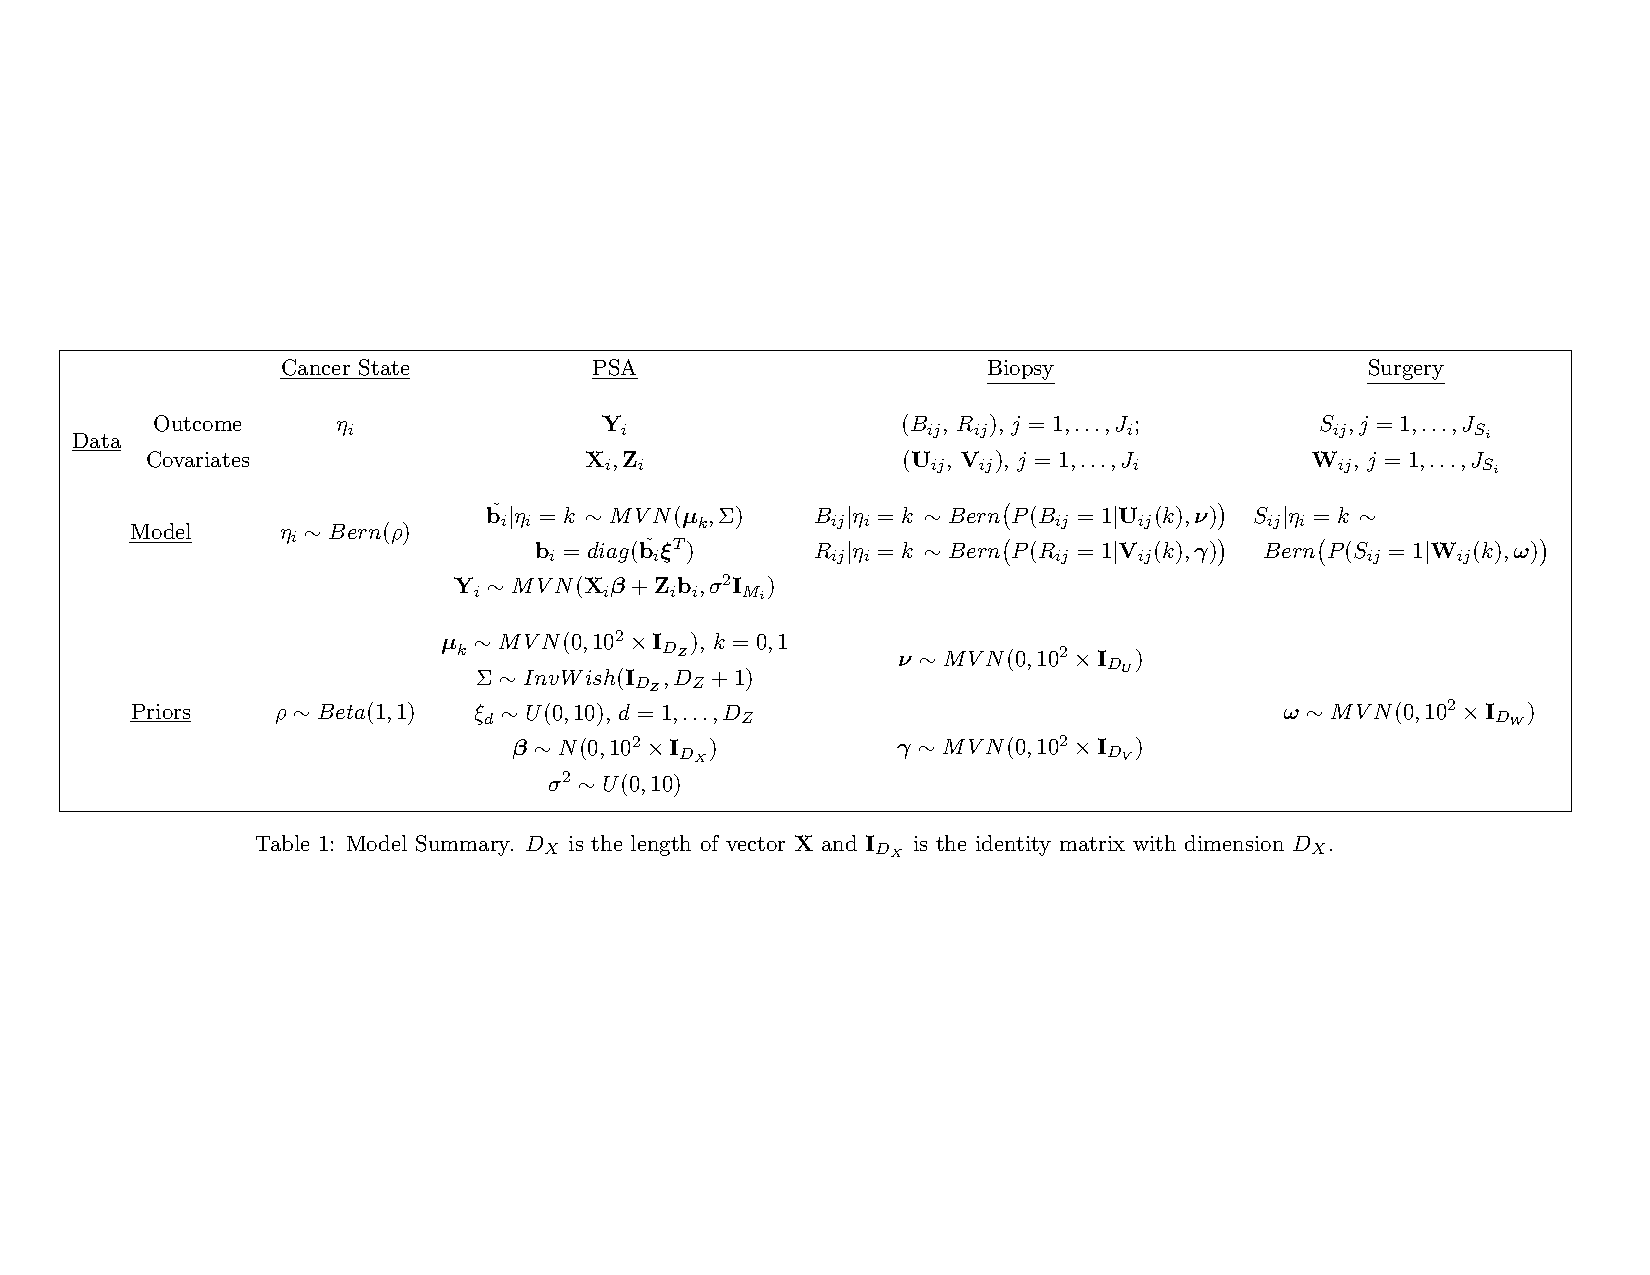
\includegraphics[width=\textwidth]{model-summary-table.pdf}
\caption{Model Summary with priors used for application to AS data. $D_X$ is the length of vector $\bmX$ and $\bmI_{D_X}$ is the identity matrix with dimension $D_X$.}
\label{fig:model-summary}
\end{center}
\end{figure}



\subsection{Results}
874 patients from the Johns Hopkins Active Surveillance cohort met the criteria for inclusion in this analysis. The number of observations and years of follow-up available for analysis are summarized in Table \ref{tab:num_obs}. Reclassification was observed in 160 patients (18$\%$). 167 patients (19$\%$) elected for surgical removal of the prostate-- 78 after experiencing reclassification-- of which 161 had post-surgery full prostate Gleason score determination available. Results of post-surgery pathologic analysis are compared to pre-surgery reclassification in Table \ref{tab:eta-vs-rc}. A total of 318 patients (36$\%$) were censored due to receiving some curative intervention, 130 (15$\%$) were lost to follow-up, and nineteen (2.2$\%$) were censored due to death. (No patients died of prostate cancer.) 407 patients (47$\%$) remained active in the program at the time of data collection for this analysis. 


\begin{table}
\begin{center}
\begin{tabular}{|c|c|c|}
\hline
 & Total $\#$ observations & Median $\#$ per patient (IQR) \\[5pt]
\hline
PSA & 10,425 & 10 (6,16)\\[5pt]
Biopsy & 2,741 & 3 (1,4)\\[5pt]
Years of follow-up & \multirow{2}{*}{4,980} & \multirow{2}{*}{5 (3,8)}\\
(prior to reclassification) & & \\[5pt]
\hline
\end{tabular}
\caption{Summary of observations and follow-up time for $n$=874 patients included in analysis.}
\label{tab:num_obs}
\end{center}
\end{table}

\begin{table}
\begin{center}
\begin{tabular}{|c|c|c|c|}
\hline
& \multicolumn{2}{|c|}{Reclassification} & \\
 & $R$=0 & $R$=1 & Total\\[5pt]
 \hline
Indolent, $\eta=0$ & 66  (69$\%$) & 17 (26$\%$) & 83 \\[5pt]
Aggressive, $\eta=1$ & 30 (31$\%$) & 48 (74$\%$) & 78\\[5pt]
 \hline 
 Total & 96 & 65 & 161\\[5pt]
\hline
\end{tabular}
\caption{Summary of post-surgery cancer state determination ($\eta$) compared to reclassification ($R$) on final biopsy with column percentages in subset of patients with true state observed ($n=161$)}
\label{tab:eta-vs-rc}
\end{center}
\end{table}


Figure \ref{fig:singles} shows the PSA and biopsy data available on a dozen patients in the cohort.  Plotting circles represent observed PSA values, with the scale given on the lefthand y-axis. Triangles represent biopsies, with open triangles indicating no biopsy in an annual interval (and, thus, no reclassification observed) and filled triangles indicating biopsy results; triangles at the bottom of the plot represent no grade reclassification while those at the top represent a Gleason score of 7 or higher on biopsy. Alongside the observed data, Figure \ref{fig:singles} also gives posterior predictions from the proposed model about each patient's true cancer state (above each plot), likely PSA trajectory, and risk of reclassification on a future biopsy (with scale given on righthand y-axis). Shaded credible intervals indicate the posterior distribution for these predictions with the darkest shading occurring at the posterior median. Note that no reclassification projections are given for those patients with grade reclassification observed, as they will not continue with biopsies.  

\begin{figure}
\begin{center}
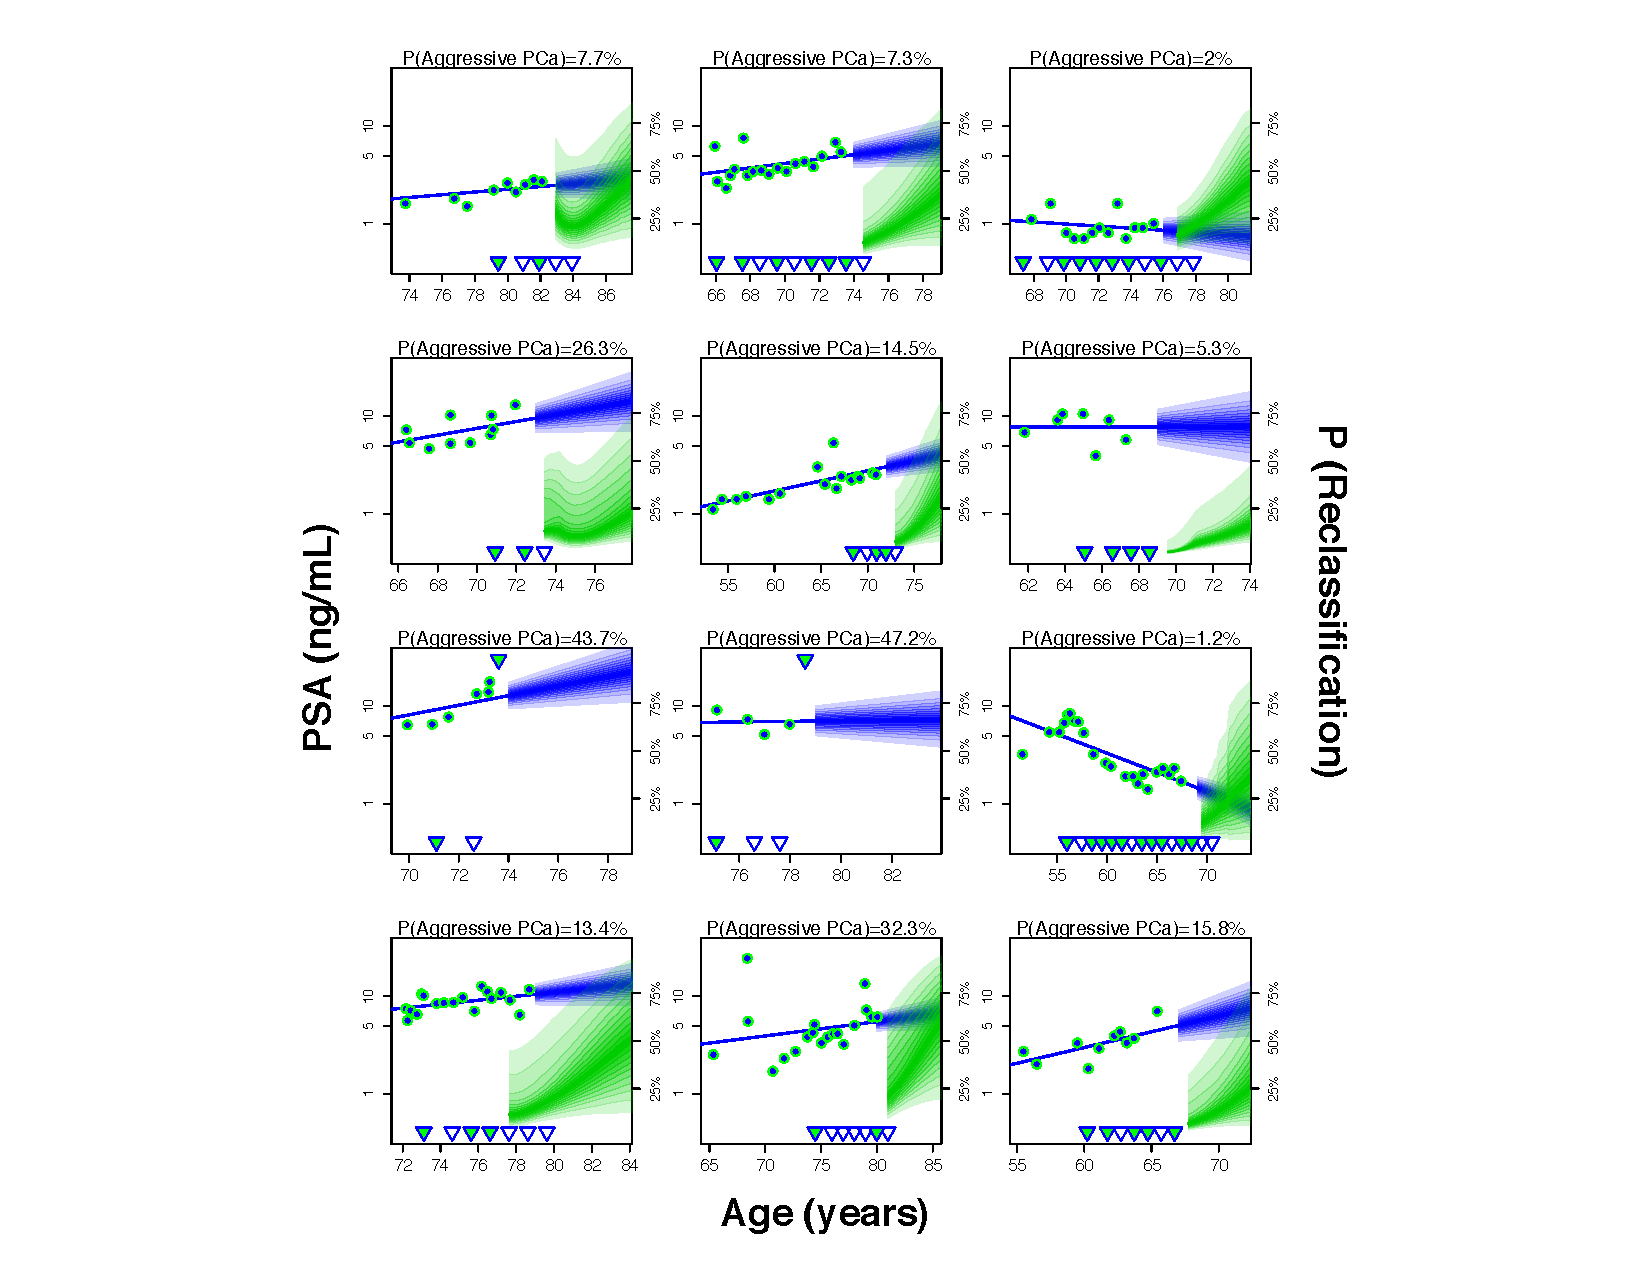
\includegraphics[width=\textwidth]{data-and-predictions.pdf}
\caption{PSA (circles) and reclassification (triangle) data for a dozen patients. Posterior probabilities of having aggressive prostate cancer are above each patient's data. Shaded intervals show posterior credible intervals around projected PSA (blue) and reclassification (green) trajectories. }
\label{fig:singles}
\end{center}
\end{figure}


The ROC curves and calibration plot in Figure \ref{fig:eta-accuracy} illustrate the proposed informative observation process (IOP) model's ability to accurately predict an individual's cancer state. The out-of-sample AUC among patients with true cancer state known is 0.75, slightly higher than the simple model which has an AUC of 0.72. In the right-hand panel, the calibration plot shows that posterior predictions of underlying aggressive cancer generally follow the observed rates (i.e., track the x=y axis), with the exception of very low risk predictions, where less data is available. In this plot, hashmarks at y=0 and y=1 show the observed cancer state for individuals against their posterior prediction on the x-axis. 
\begin{figure}
\begin{center}
\begin{subfigure}[b]{0.45\textwidth}
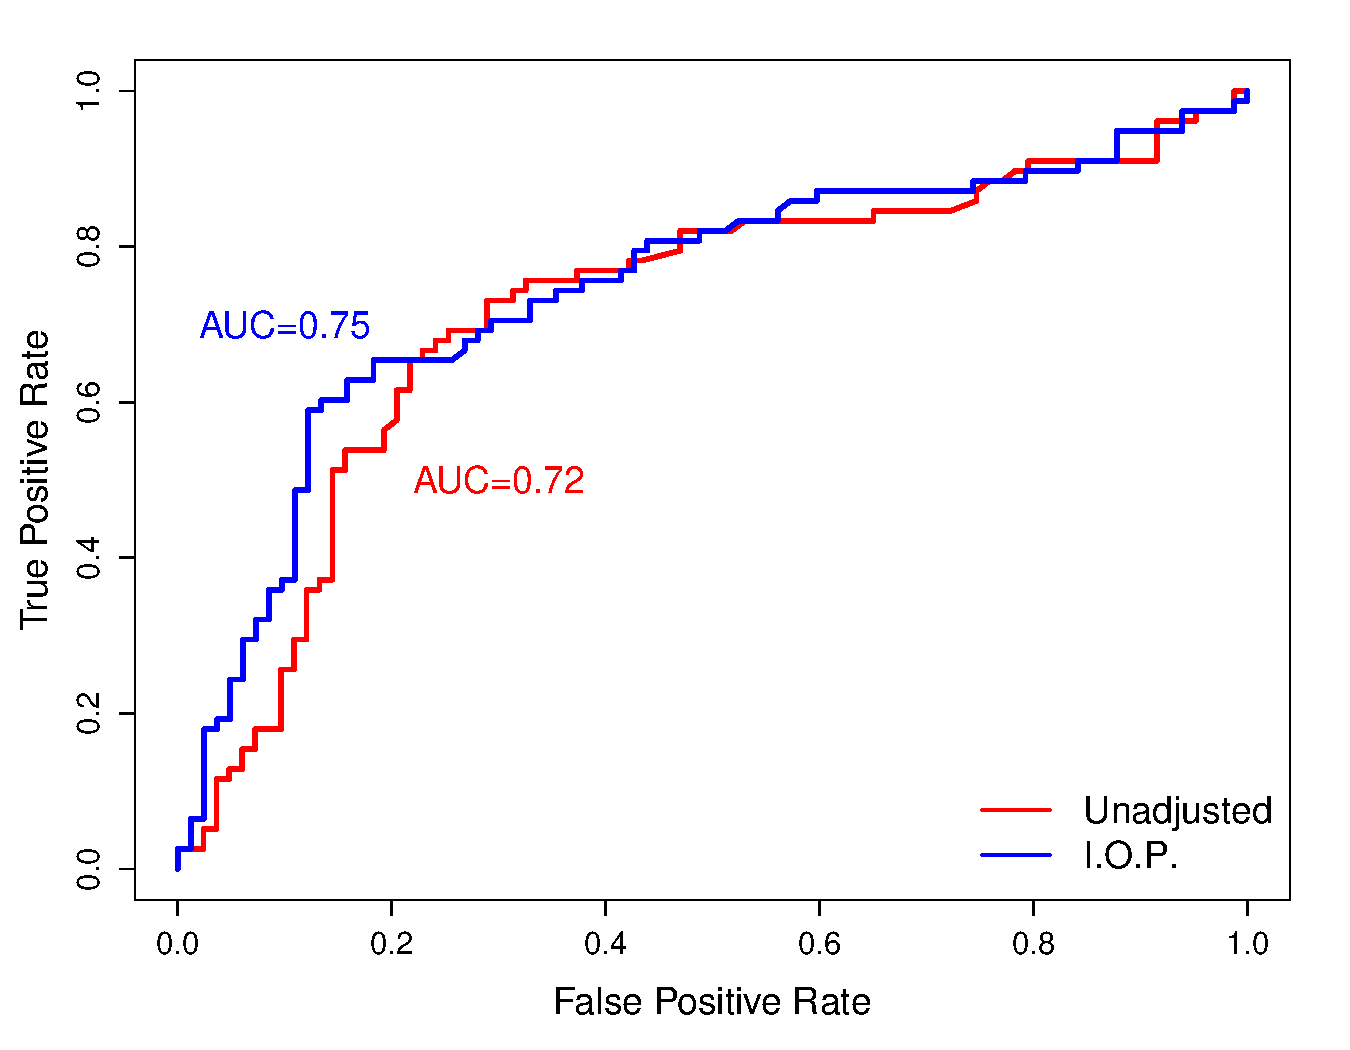
\includegraphics[width=\textwidth]{pred-vs-obs-eta-roc}
%\caption{}
\label{fig:roc}
\end{subfigure}
\begin{subfigure}[b]{0.45\textwidth}
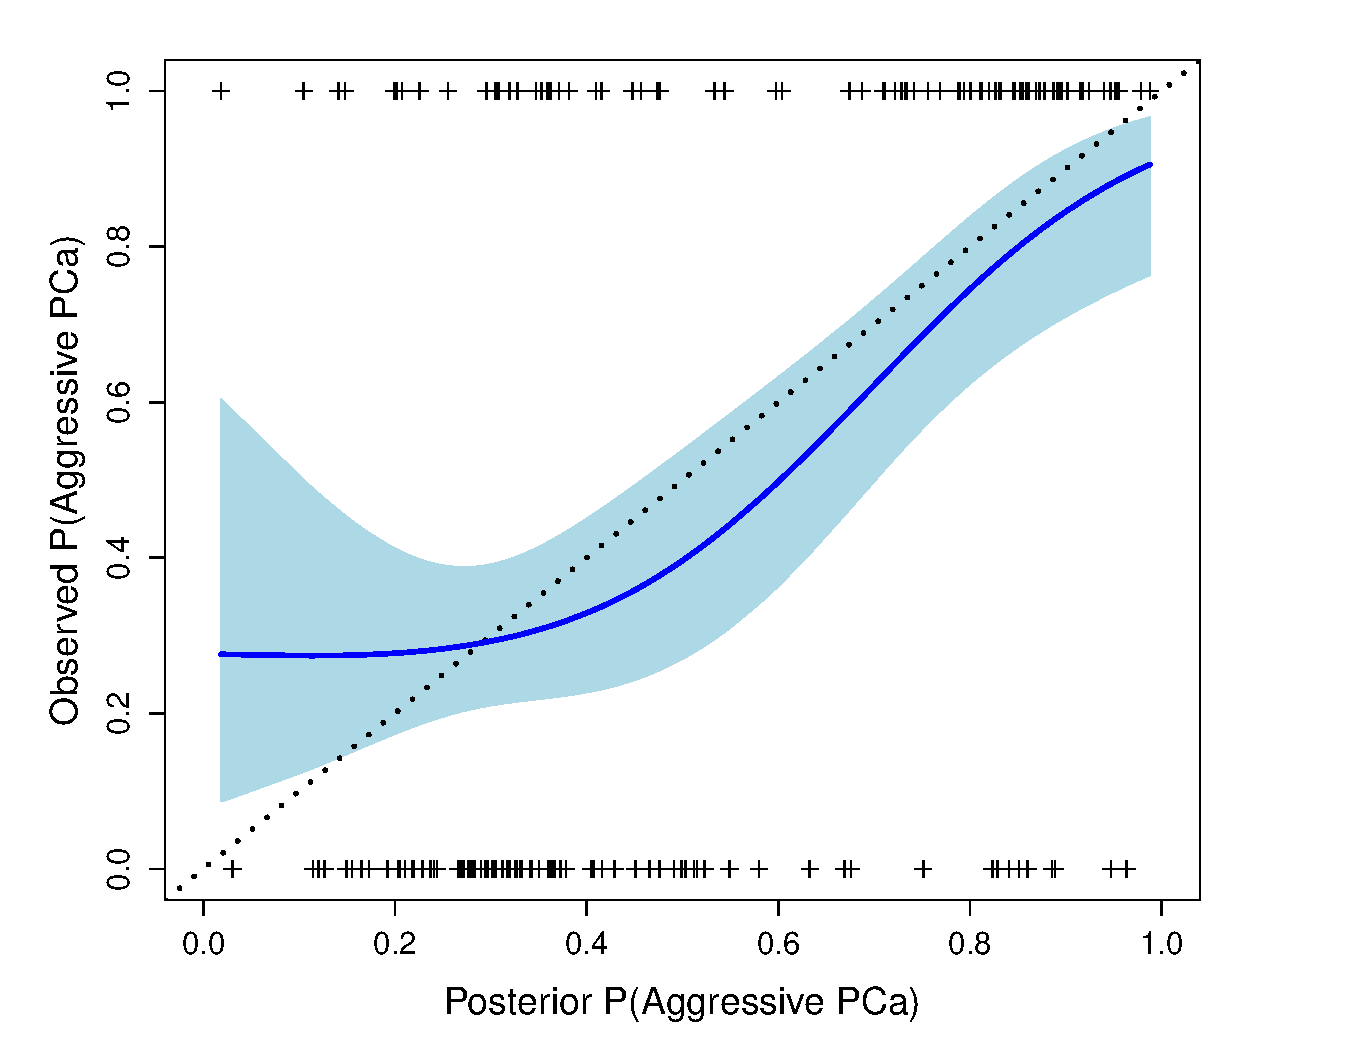
\includegraphics[width=\textwidth]{pred-vs-obs-eta}
%\caption{}
\label{fig:calibrartion-eta}
\end{subfigure}
\caption{ROC curve (left panel) and calibration plot (right panel) for predictions of underlying cancer state, $\eta$, among those with true state observed}
\label{fig:eta-accuracy}
\end{center}
\end{figure}


Calibration plots for posterior predictions of biopsy, reclassification, and surgery are given in Figure \ref{fig:calibration-all-bx}. Overall, posterior probabilities reflect observed rates of each outcome, especially in ranges with more data. Posterior predictions appear less accurate for reclassification but we note that the vast majority of person-years (87$\%$) have a predicted risk of reclassification below 10$\%$, where the model fits well. We suspect that the lack of strong predictors of reclassification limited our ability to accurately predict risk at higher ranges. 

\begin{figure}
\begin{center}
\begin{subfigure}[b]{0.5\textwidth}
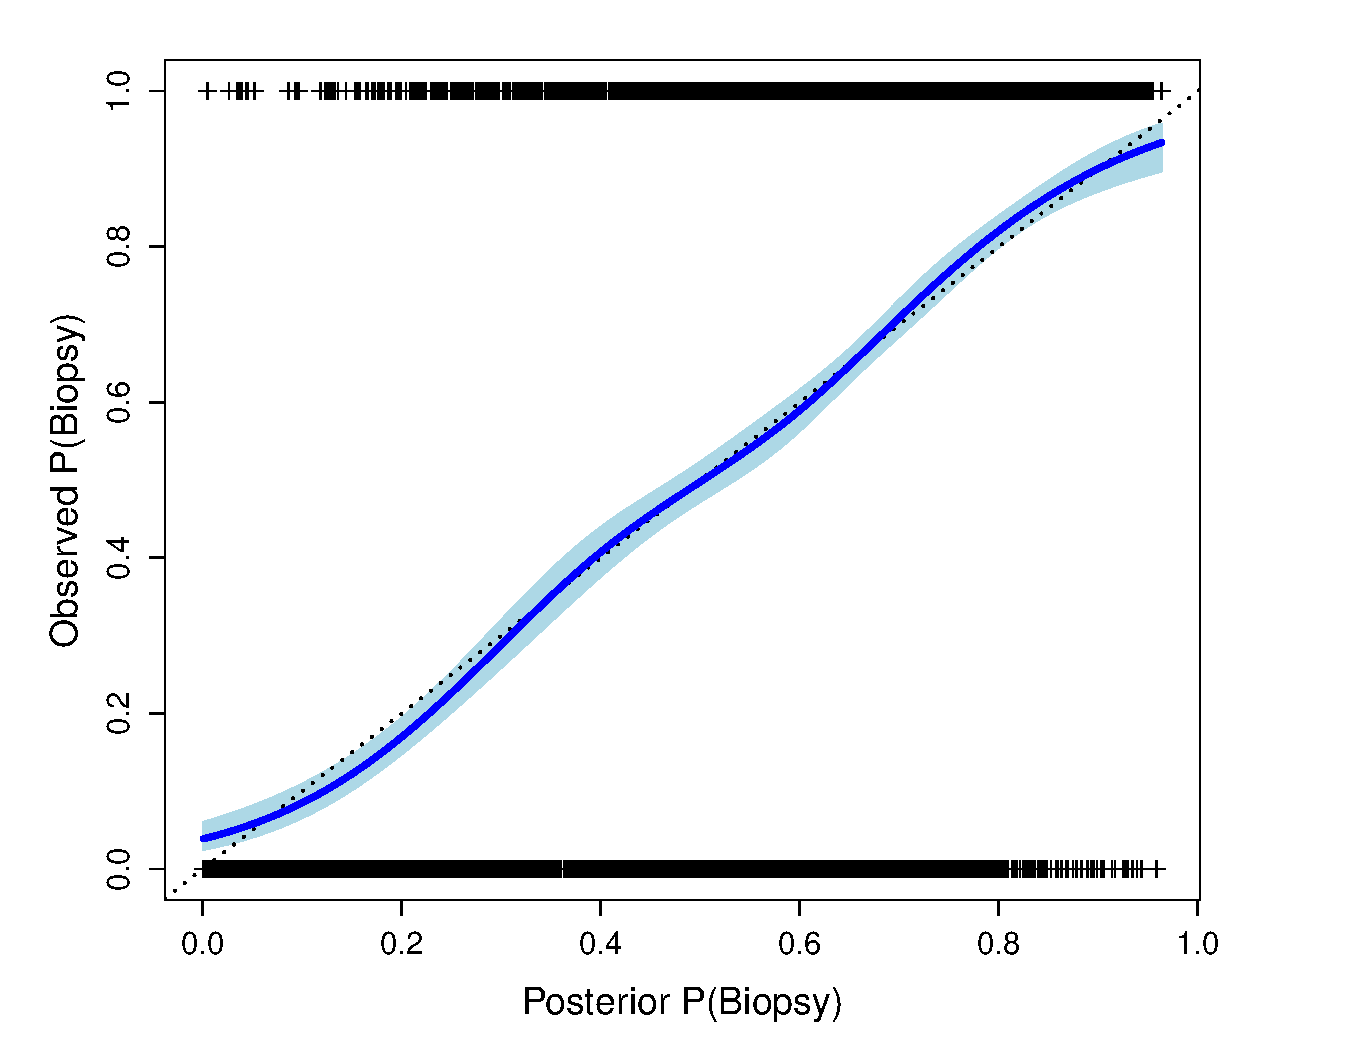
\includegraphics[width=\textwidth]{pred-vs-obs-bx.pdf}
%\caption{}
%\label{fig:calibration-bx}
\end{subfigure}
\begin{subfigure}[b]{0.5\textwidth}
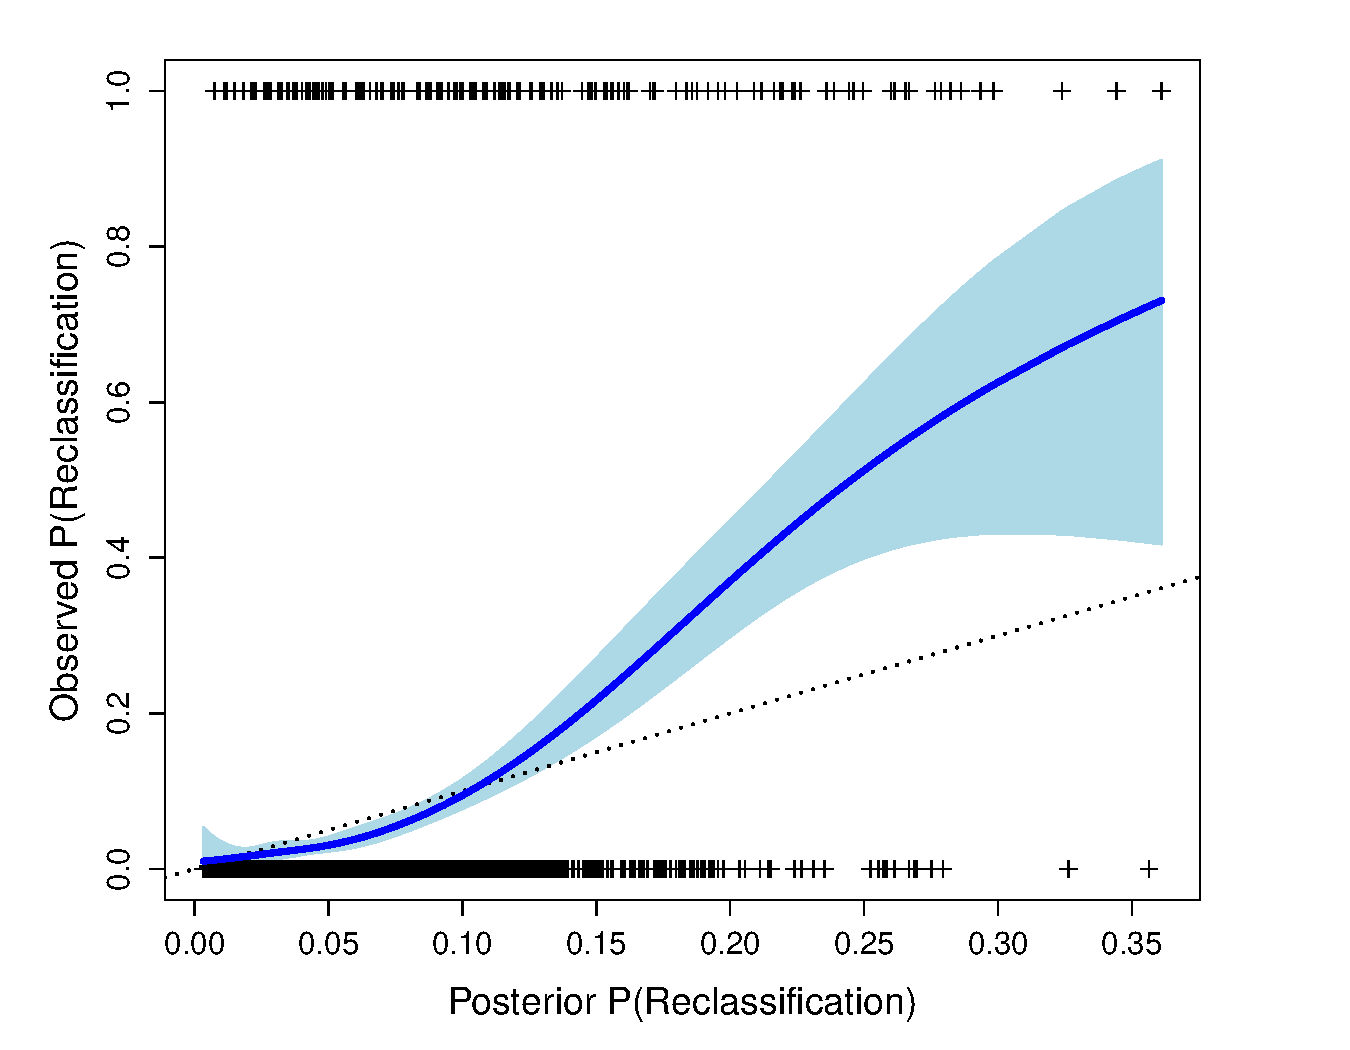
\includegraphics[width=\textwidth]{pred-vs-obs-rc.pdf}
%\caption{}
%\label{fig:calibrartion-rc}
\end{subfigure}
\begin{subfigure}[b]{0.5\textwidth}
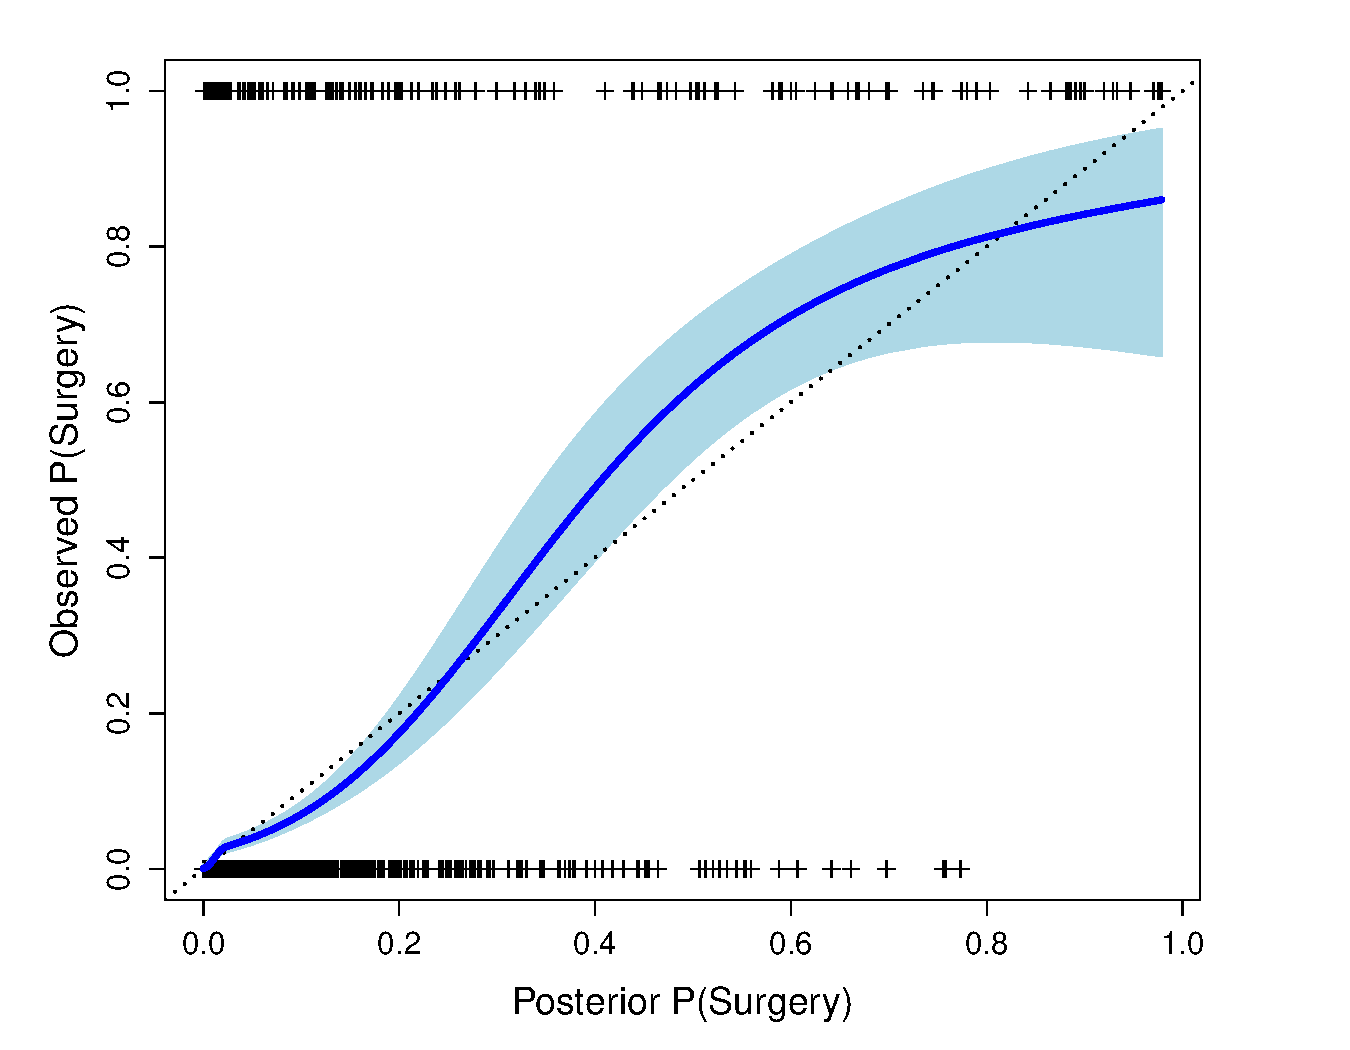
\includegraphics[width=\textwidth]{pred-vs-obs-rrp.pdf}
%\caption{}
%\label{fig:calibrartion-rrp}
\end{subfigure}
\caption{Calibration plots for predicting biopsies (top), reclassification (middle), and surgery (bottom) in annual intervals for all patients} 
\label{fig:calibration-all-bx}
\end{center}
\end{figure}


The model was also fit with informative priors on the effect of partially latent cancer state on the risk of surgery in order to assess robustness of posterior predictions to prior specification and under the concern that the relationship between an outcome's missingness and its value may not be identifiable from the likelihood alone. A range of informative priors (e.g., aggressive cancer increases, does not affect, or decreases risk of surgery) were found to have no impact on the model's predictive accuracy, indicating that identifiability of informative surgery parameters does not depend on proper priors. %(For this reason, results are not discussed here in more detail.) 
%To assure identifiability of the informative surgery parameters, a

%%put in all the graphs

\section{Discussion}
In this paper, we have presented a hierarchical Bayesian joint model for predicting latent cancer state among low risk prostate cancer patients from repeated biopsy and PSA results as well as information available in the observation process. While multiple models exist for providing individualized predictions of biopsy results for this population, this paper is the first to predict the outcome of chief concern- the true underlying state of an individual's prostate cancer. This approach demonstrates the potential for precision medicine approaches that provide individualized predictions of latent health states and trajectories, instead of focusing only on error-prone measurements of the health state. 
%Within a hierarchical latent class framework, our model also predicts likely outcomes of biopsy and PSA tests, which can guide decision-making about future tests.

The proposed prediction model also exemplifies the statistical underpinnings of a learning health care system \cite{IOM2012,Smith2013}, a system with the ability to continuously integrate patient data and medical knowledge to optimize patient care. As more patients enroll in the Johns Hopkins Active Surveillance cohort, and as more information is collected on existing patients, our ability to predict underlying health states and the likely trajectory of clinical outcomes is likely to improve. Furthermore, online updating methods can be used to obtain real-time prediction updates based on the most current information in order to inform decision-making in a clinical setting. For example, see the accompanying technical report for an importance sampling algorithm that provides fast predictions (REF). %At this time, real-time updating is only available for individual-level parameters; standard Bayesian estimation procedures can be routinely performed on refreshed data to update all  model parameters. 

% the pace of advances in medical research demand that effective statistical frameworks be responsive to discoveries by readily reflecting the most up-to-date knowledge

The proposed prediction model that targets the latent cancer state can be easily modified in response to the availability of additional data or advancement in scientific understanding. In particular, the proposed prediction model could also be extended to allow for time-varying latent states if information on the rate of disease progression in this population were available. Current model specification assumes that  an individual's cancer categorization does not change over the time period under surveillance, an expectation supported by Porten et al. (2011)\nocite{Porten2011} who showed that upgrading, particularly early on in active surveillance, is mostly due to misclassification at diagnosis rather than disease progression. This assumption is also necessary as a time-varying latent state would be nonindentifiable without additional assumptions on the rates of disease progression. For example, a recent natural history approach to modeling underlying prostate cancer state by Inoue et al. (2014)\nocite{Inoue2014}, suggested a rate of disease progression in the Johns Hopkins AS cohort of 12-14$\%$ within a decade of enrollment. While these estimates were strongly dependent on prior specification, continued research on this question could inform a future extension to time-varying cancer state.


%Likewise, estimation of a dynamic latent state in the current data would rely heavily on modeling assumptions and prior specification for identifiability. In the future, increased scientific consensus on rates of progression, coupled with clinical measures of disease state, may enable  prediction of a time-varying cancer state with greater confidence.


This model can also readily accommodate new predictors or outcomes. When, for example, a genetic marker for prostate cancer risk is identified, the probability distribution for latent state could be stratified by subgroups defined by this marker. Or, if additional biopsy results, such as the number of positive cores or maximum percent cancer involvement, were found to be predictive of true cancer state, regressions of these repeated outcome measures of latent class could also be included in the joint model. In the case that some measurements are not available for all patients, the proposed framework is also able to adjust for informative observation of predictors and outcomes. As a result, the prediction model presented here can continue to provide the most advanced decision support to physicians and patients as new knowledge and expertise is acquired.


%This paper demonstrates a statistical modeling approach to support individualized prediction of a latent health state within the broader setting of a learning health systems. Similar examples... 



\bibliographystyle{plain}
\bibliography{/Users/ryc/Dropbox/inhealth/inhealth-bib}
\end{document}

\section{Appendix}
\subsection{Importance sampling procedure}
For the purposes of this appendix, we introduce the following abbreviated form of the joint posterior given in \ref{eq:post-inf}: 
\begin{equation}
p(\theta,b_{1:n}|y_{1:n})\propto\prod_{i=1}^{n}[f(y_{i}|b_{i},\theta)g(b_{i}|\theta)]\pi(\theta)\label{eq:posterior_n}
\end{equation}
 Where $y_{i}$ is the vector of measurements for patient $i$, $y_{1:n}$ is the list of measurements for the first $n$ patients, $b_{i}$ is a vector of latent variables for patient $i$, $b_{1:n}$ is a list of latent variables for the first $n$ patients, $\theta$ contains the population-level parameters, $\pi$ is the prior for $\theta$, and $f$ and $g$ are multivariate distributions coming from the model likelihood in \ref{eq:lik-inf}. We first illustrate how importance weighting can be used to quickly estimate latent variables for a new patient before showing how similar calculations can be done to incorporate newly measured data on existing patients in real-time.
 
\subsubsection{Fast predictions for a new patient}
 Here, we focus on obtaining posteriors of latent variables for a new patient (indexed by $n+1$). Our ultimate goal is to calculate expectations with respect to the posterior distribution based on all $n+1$ patients (i.e. $p(\theta,b_{1:(n+1)}|y_{1:(n+1)})$). While we cannot immediately draw from this distribution, we can evaluate a function that is proportional to its density (Equation \ref{eq:posterior_n}). To carry out importance sampling, we need to choose a proposal distribution $q$ from which to generate candidate values of $(\theta,b_{1:(n+1)})$. We use the posterior distribution based on the first $n$ patients as our proposal distribution. This approach is analogous to a one-step particle filter \cite{Bishop2006}.
\begin{eqnarray*}
q(\theta,b_{1:(n+1)}) & := & g(b_{n+1}|\theta)p(\theta,b_{1:n}|y_{1:n})
\end{eqnarray*}

Practically, this consists of taking $J$ draws of $\theta$ and $b_{1:n}$ from the previously fitted posterior in Eq \ref{eq:posterior_n}. Then, conditional on $\theta$, we draw $b_{n+1}$ from the distribution $g$. We index each of the resulting draws as $(\theta^{(j)},b_{1:(n+1)}^{(j)})$, with $j=1,\dots,J$. The importance weights $w_{j}$ are then proportional to 
\begin{eqnarray}
w^{(j)} & \propto & \frac{p(\theta^{(j)},b_{1:(n+1)}^{(j)}|y_{1:(n+1)})}{q(\theta^{(j)},b_{1:(n+1)}^{(j)})} \nonumber \\
 & \propto & \frac{\prod_{i=1}^{n+1}[f(y_{i}|b_{i}^{(j)},\theta^{(j)})g(b_{i}^{(j)}|\theta^{(j)})]\pi(\theta^{(j)})}{g(b_{n+1}^{(j)}|\theta^{(j)})\prod_{i=1}^{n}[f(y_{i}|b_{i}^{(j)},\theta^{(j)})g(b_{i}|\theta^{(j)})]\pi(\theta^{(j)})} \nonumber \\
\label{eq:importance-weights}
 & = & f(y_{i}|b_{i}^{(j)},\theta^{(j)})
\end{eqnarray}

The final weights $w^{(j)}$ are standardized to sum to 1. The new posterior for $(\theta,b_{1:(n+1)})$ can then be represented as the mixture distribution satisfying $P(\theta=\theta^{(j)},b_{1:(n+1)}=b_{1:(n+1)}^{(j)})=w^{(j)}$. A posterior mean for $b_{(n+1)}$ can be calculated as $\sum_{j=1}^{J}w^{(j)}b_{(n+1)}^{(j)}$. The unstandardized weights can also be used in a rejection sampling procedure, although we found this approach to be less computationally efficient than importance sampling for our scenario.


\subsubsection{Fast predictions for existing patients with new data}

For a patient $k$ with existing data, where we already have a posterior sample for their latent variable values, we instead use this posterior as our proposal distribution $q(\theta^{(j)},b_{1:n}^{(j)})$, with $i\leq n$. Let $y_{1:n}^{k+}$ refer to the data set after incorporating new data on patient $k$, where $y_{i}^{+}=y_{i}$ if $k\neq i$. The importance weights in Equation \ref{eq:importance-weights} then simplify to
\begin{eqnarray*}
w^{(j)} & \propto & \frac{p(\theta^{(j)},b_{1:n}^{(j)}|y_{1:n}^{+})}{q(\theta^{(j)},b_{1:n}^{(j)})}\\
 & \propto & \frac{\prod_{i=1}^{n}[f(\ensuremath{y_{i}^{+}}|b_{i}^{(j)},\theta^{(j)})g(b_{i}^{(j)}|\theta^{(j)})]\pi(\theta^{(j)})}{\prod_{i=1}^{n}[f(\ensuremath{ y_{i} }|b_{i}^{(j)},\theta^{(j)})g(b_{i}^{(j)}|\theta^{(j)})]\pi(\theta^{(j)})}\\
 & = & \frac{f(\ensuremath{ y_{k}^{+}} |b_{ k }^{(j)},\theta^{(j)})}{f(\ensuremath{ y_{k}} |b_{k}^{(j)},\theta^{(j)})}
\end{eqnarray*}

Let $L_{k}$ denote that number of measurements for which we've previously fit a posterior for $b_{k}$, and let $N_{k}$ denote the number of new measurements we wish to incorporate into this posterior. Then, $y_{k}^{+}$ can be expressed as the vector $y_{k}^{+}=(y_{k[1]},y_{k[2]},\dots y_{k[L_{k}]},y_{k[L_{k}+1]}^{+},\dots y_{k[L_{k}+N_{k}]}^{+})$, where $y_{k[l]}^{+}$ is the $l^{th}$ measurement from patient $k$. If the repeated measures for each patient are independent conditional on $b_{i}$, as is the case in the proposed model, then the above ratio reduces to

\begin{eqnarray*}
w^{(j)} & \propto & \frac{\prod_{l=1}^{L_{k}+N_{k}}f(\ensuremath{ y_{k[l]}^{+}} |b_{k}^{(j)},\theta^{(j)})}{\prod_{l=1}^{L_{i}}f(\ensuremath{y_{k[l]}} |b_{ k}^{(j)},\theta^{(j)})}\\
 & = & \prod_{l=L_{k}+1}^{L_{k}+N_{k}}f(\ensuremath{y_{k[l]}^{+}}|b_{k}^{(j)},\theta^{(j)})
\end{eqnarray*}


We then proceed as above to get a re-weighted posterior for the latent variables of patient $k$. 


%\end{document}



Posterior estimates from the mixed effects model for PSA are displayed in Figure \ref{fig:lme}. In this plot, each plotting circle represents the scaled random intercept (x-axis) and slope (y-axis) estimates for a single patient. Filled circles represent patients for whom the true cancer state was observed, with red indicating potentially lethal cancer found after surgery and green indicating a determination of indolent cancer. The color of open circles reflects the posterior probability of aggressive cancer, ranging from low (green) to high (red), among patients for whom true state was not observed. Finally, credible ellipses show the posterior mean and covariance of random effects for individuals in each partially latent class. We see that there is a fair amount of overlap in these intervals, indicating that PSA level and trajectory does not provide information about the true state for most patients. PSA  is more informative, however, for patients with particularly high or low levels and trajectories. 

\begin{figure}
\begin{center}
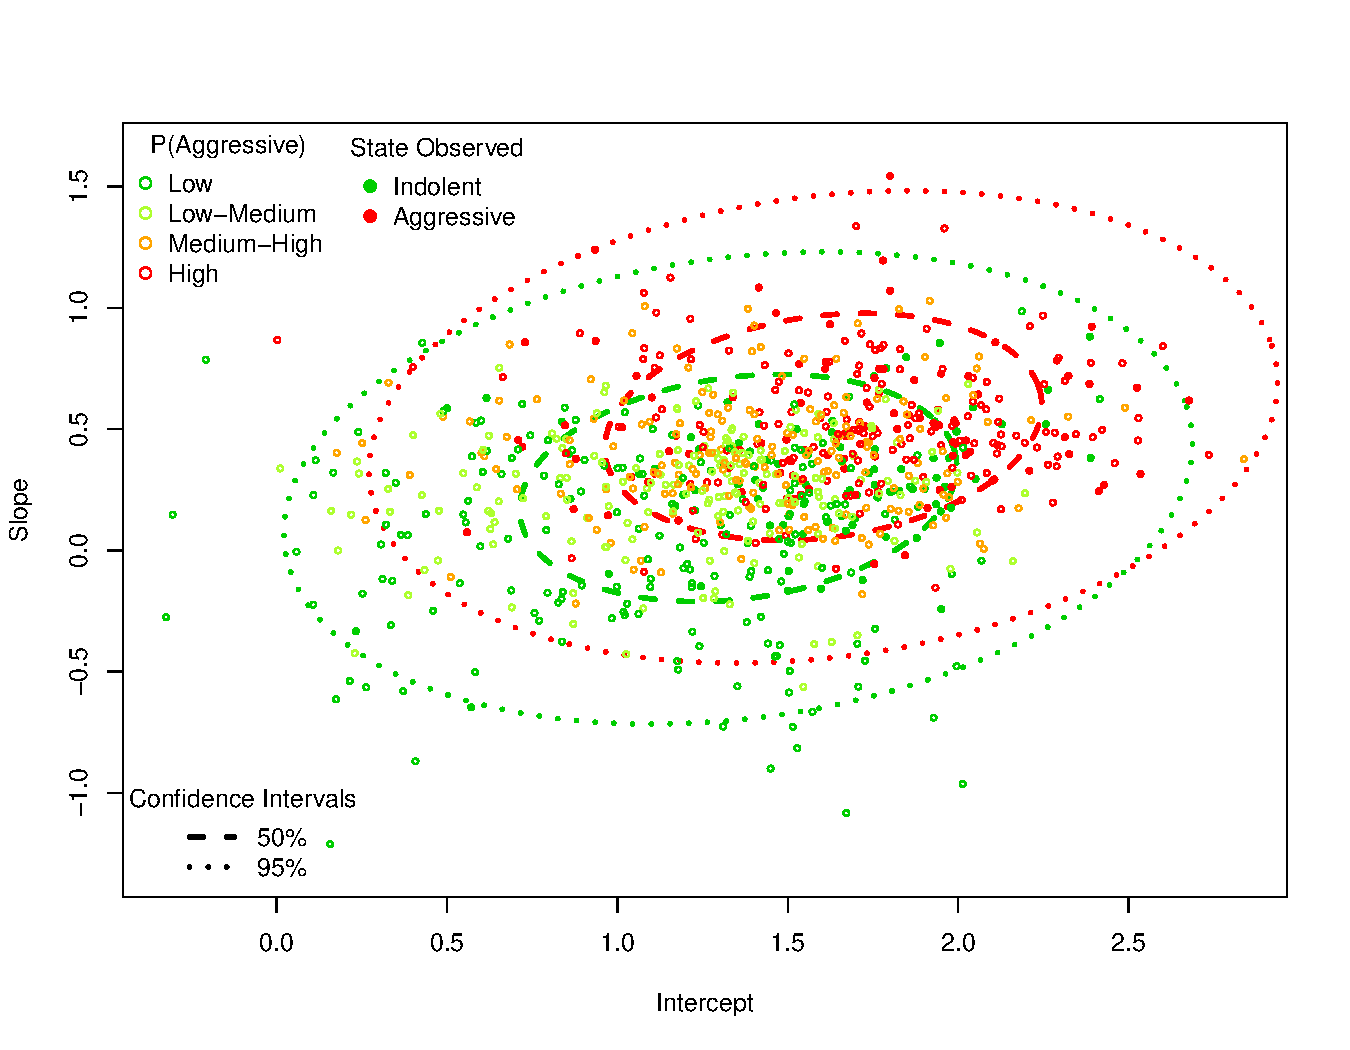
\includegraphics[width=0.8\textwidth]{random-effect-est.pdf}
\caption{Random effects estimates from stratified mixed effects model for PSA.}
\label{fig:lme}
\end{center}
\end{figure}





\section{Fast, individualized posterior estimates for new data}
For the proposed prediction model to be most useful in a clinical setting, it is necessary to be able to update posterior estimates quickly  to incorporate new biopsy or PSA results during a patient's visit. This precludes re-running the full MCMC to obtain updated posteriors of patient-specific variables. Instead, we use importance sampling \cite{Bishop2006} to obtain rapid prediction updates. After obtaining posterior estimates using current data, importance sampling to update these estimates for either a new patient or new data on an existing patient requires three steps: generating proposal values for the latent variables to be updated, calculating weights for proposed values, and weighting proposed values to estimate an updated posterior.

In order to generate proposal values for importance sampling for new patients without previous predictions, we start with samples of population-level parameters from the full joint posterior (Equation \ref{eq:post-inf}) based on previously observed data. Then, for each draw, we generate proposed values for patient-specific latent variables (true state, $\eta$, and random effects, $\bmb$) from their conditional posteriors. For patients with existing predictions that only need to be updated, posterior samples of latent variables based on earlier observations can be used as proposal values. Next, the importance weights for proposed values are proportional to the conditional likelihood of all patient data given population-level parameters and proposed latent variables. The weighted proposal distribution then constitutes the updated posterior for patient-specific latent variables. This particular importance sampling procedure can be more specifically described as a one-step version of a sequential importance resampler, also known as a particle filter \cite{Bishop2006}. We give further details of the proposed particle filter in the Appendix. Accompanying code is available at \texttt{http://github.com/rycoley/XXX}.


For implementation in clinical practice, proposals for new patients can be re-generated prior to actually observing new data, so that only weight calculating and re-weighting of the proposal distribution needs to be done in real-time. Then, predictions for each patient can be obtained in a matter of seconds. By random chance, some patients will have data such that very few of the pre-generated proposed latent values will receive high weights; this can cause instability in posterior means. However, such scenarios can be detected by monitoring the effective size of the posterior sample, also known as the effective number of particles. When this number drops below a pre-specified threshold (e.g., 500), the procedure can be repeated with a larger set of pre-generated proposals. 

We assessed performance of the proposed importance sampling approach in the Johns Hopkins Active Surveillance cohort data. We compared the posterior probability of aggressive cancer, $P(\eta_i)$, obtained from MCMC performed in \texttt{JAGS} under two scenarios for each patient in the cohort without true cancer state observed. First, we examine agreement between the two models when each patient is completely new, that is, MCMC is performed in the absence of any of their data and, then, the particle filter is used to predict their true cancer using all of their available data. Second, we consider the scenario where additional data is observed for a patient who has already been included in the prediction model. Specifically, MCMC is performed including all data from a patient up until their penultimate biopsy (and all data from all other patients). Then, the particle filter is used to predict their true cancer state using the remaining data for that patient. 

Results of this comparison are shown in Figure \ref{fig:jags-vs-pf}. On the left, we see agreement between methods when a patient is newly introduced. Here, correlation between posterior probabilities from \texttt{JAGS} and the particle filter is 0.9950. The righthand panel compares posterior predictions between the \texttt{JAGS} fit and the particle filter for each patient when the final biopsy is included. In this scenario, the correlation is 0.XX. From these results, we conclude that the particle filter is an appropriate substitute for full MCMC runs in order to provide real-time updates in a clinical setting. 

\begin{figure}
\begin{center}
\begin{subfigure}[b]{0.45\textwidth}
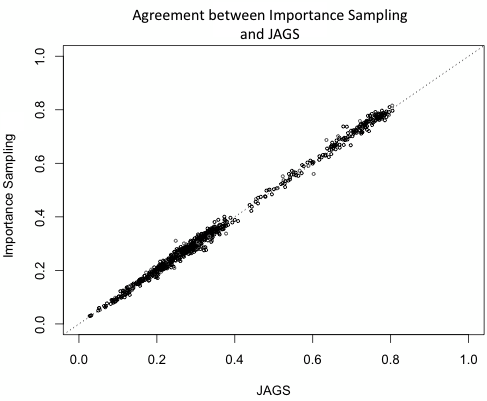
\includegraphics[width=\textwidth]{2015-07-01_compare_fits_manual-edit}
\end{subfigure}
\begin{subfigure}[b]{0.45\textwidth}
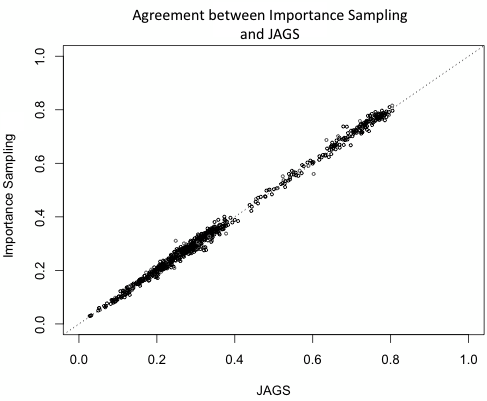
\includegraphics[width=\textwidth]{2015-07-01_compare_fits_manual-edit}
\end{subfigure}
\caption{Agreement between importance sampling and JAGS posterior predictions of prostate cancer state for a new patient (left panel) and for a patient with updated data (right panel). (Placeholder figures) }
\label{fig:jags-vs-pf}
\end{center}
\end{figure}


The proposed importance sampling approach still requires the periodic use of MCMC to perform full model updates, similar to the procedure described in Lee and Chia (2002)\nocite{Lee2002}. While fully online updating of all posteriors (that is, updating not dependent on periodic MCMC) via sequential importance resampling would be ideal, such online methods are known to suffer from the problem of degeneracy when the model includes static parameters (such as the population-level parameters in our model), as explained in Andrieu et al. (2005, section II)\nocite{Andrieu2005}.

